%  LaTeX support: latex@mdpi.com
%  For support, please attach all files needed for compiling as well as the log file, and specify your operating system, LaTeX version, and LaTeX editor.

%=================================================================
\documentclass[jimaging,article,submit,pdftex,moreauthors]{Definitions/mdpi}

% Figures live at repository root; this manuscript is compiled from draft/.
\graphicspath{{../}}

%=================================================================
% MDPI internal commands - do not modify
\firstpage{1}
\makeatletter
\setcounter{page}{\@firstpage}
\makeatother
\pubvolume{1}
\issuenum{1}
\articlenumber{0}
\pubyear{2026}
\copyrightyear{2026}
\datereceived{}
\daterevised{}
\dateaccepted{}
\datepublished{}

%=================================================================
\usepackage{algorithm}
\usepackage{algpseudocode}

%=================================================================
% Anonymous manuscript variant: author identities, contribution
% statements, and acknowledgments omitted (for double-blind or similar use).
%=================================================================
% Title
\Title{Hyperelastic Regularization for Reducing Folding in Transformer-Based Brain MRI Registration}

\Author{[Author names withheld]}

\AuthorNames{[Withheld]}

\address{%
}

\corres{}

% Abstract
\abstract{\textbf{Background:} Transformer-based deformable brain MRI registration achieves high overlap accuracy, but predicted displacement fields can contain voxels with non-positive Jacobian determinant---local foldings that violate the diffeomorphism assumption required by tensor-based morphometry and atlas-fusion segmentation workflows. \textbf{Methods:} We introduce HypEReg, a non-linear hyperelastic regularizer that acts directly on the Jacobian determinant of the predicted displacement field. HypEReg couples a clamped-rational volume-distortion penalty \((\det J_\phi-1)^2/\max(\det J_\phi,\epsilon)\) with an explicit per-voxel anti-folding hinge \([\max(0,\epsilon-\det J_\phi)]^2\), integrated as a purely loss-side module into a TransMorph backbone with no inference-graph modifications. \textbf{Results:} On the IXI atlas-to-subject benchmark (115 test subjects), HypEReg-TransMorph maintains grouped Dice (0.7537) while reducing the \(\det(J_\phi)\le 0\) voxel ratio from \(1.502\times10^{-2}\) (TransMorph) to \(1.5\times10^{-5}\), with identical per-case runtime and parameter count to the unregularized baseline. In strict zero-shot transfer to OASIS Learn2Reg test pairs (no fine-tuning), HypEReg-TransMorph achieves Dice 0.7756 with a \(\det(J_\phi)\le 0\) ratio of \(7.6\times10^{-5}\), roughly two orders of magnitude below plain TransMorph zero-shot (Dice 0.7691; ratio \(9.6\times10^{-3}\)); downstream multi-atlas label fusion further confirms the practical benefit of fold suppression (fused Dice 0.8271 vs.\ 0.8201 for TransMorph). \textbf{Conclusions:} Determinant-level, non-linear hyperelastic regularization substantially suppresses folding in Transformer dense-flow brain MRI registration while preserving alignment accuracy and adding zero inference cost, providing a practical drop-in regularization strategy for morphometry-ready deformable registration.}

\keyword{deformable image registration; brain MRI; TransMorph; Jacobian determinant; Jacobian-aware regularization; hyperelastic regularization; folding suppression; diffeomorphic registration}

%%%%%%%%%%%%%%%%%%%%%%%%%%%%%%%%%%%%%%%%%%
\begin{document}

%%%%%%%%%%%%%%%%%%%%%%%%%%%%%%%%%%%%%%%%%%
\section{Introduction}

Deformable registration is a foundational primitive of computational neuroimaging. Atlas propagation, voxel-wise morphometry, and longitudinal monitoring of disease progression all rely on the assumption that a smooth, invertible mapping can be recovered between a moving anatomy and a target reference. Classical iterative formulations, exemplified by SyN and other diffeomorphic frameworks, build this assumption into the optimization objective by explicitly constraining transformation smoothness and invertibility \cite{avants2008ants,rueckert1999nonrigid,ashburner1999morphometry}. The deformation fields that these methods produce are well behaved, but each registration is solved as an iterative inverse problem and is therefore expensive to deploy at population scale.

Learning-based registration was introduced largely to remove this throughput bottleneck. Following the introduction of VoxelMorph and related convolutional architectures \cite{balakrishnan2019voxelmorph,kim2021cyclemorph}, a single forward pass through a trained network can produce a dense displacement field in a fraction of a second, with overlap accuracy that often matches or exceeds classical baselines. Probabilistic diffeomorphic variants further stabilize the predicted deformations \cite{dalca2019probreg}, and the recent adoption of Transformer encoders has improved long-range contextual modelling for volumetric registration \cite{chen2022transmorph,liu2021swin}. Across these advances, however, one issue has proved persistent: when displacement is predicted directly and without an intrinsic regularity prior, the resulting deformation is not guaranteed to be diffeomorphic. Local foldings---voxels at which \(\det J_\phi\le 0\)---appear systematically in the output of unconstrained Transformer registration networks, regardless of how high the Dice score happens to be.

This is more than a mathematical inconvenience. The Jacobian determinant is itself the quantity reported in tensor-based morphometry (TBM) and longitudinal volume-change studies, and is central to imaging endpoints in multiple neuroimaging workflows. When local foldings (\(\det J_\phi\le 0\)) appear in a deformation field, corresponding voxels report negative or undefined volume change, biasing voxel-wise statistical maps. Constraining the predicted deformation to be near-diffeomorphic at training time therefore has direct implications for the trustworthiness of Jacobian-based analyses.

The deep-learning literature has approached this regularity problem from several angles. Mok and Chung \cite{mok2020fast} introduced a selective Jacobian-determinant penalty that activates only on candidate folded voxels (\(\det J\le 0\)) inside a diffeomorphic CNN; this is the conceptual antecedent of the anti-folding term used in the present work. Hering et al.\ \cite{hering2021lung} embedded a Burger--Modersitzki--Ruthotto-style volume-change penalty alongside a curvature regularizer in a CNN-based lung-CT registration pipeline, and Zou et al.\ \cite{zou2023conformal} explored conformal-invariant hyperelastic energies in the same lung-CT setting. Inverse-consistency formulations such as ICON \cite{greer2021icon} and GradICON \cite{tian2023gradicon} encourage cycle agreement between forward and backward warps, while hierarchical constructions such as LapIRN \cite{mok2020lapirn} compose the deformation across multiple Laplacian scales. To our knowledge, coupling a non-linear determinant-level hyperelastic-style regularizer of the HypEReg form with a Transformer-based dense-flow backbone and subject-level paired inferential statistics, as we do here, has not been previously reported; it is also in this high-capacity setting that folding artefacts are often most visible.

In this paper, we develop HypEReg, a non-linear hyperelastic regularizer derived from the Burger--Modersitzki--Ruthotto (BMR) energy \cite{burger2013hyperelastic} but redesigned for stochastic optimization in a deep-learning context. HypEReg combines a clamped-rational volume-distortion penalty \((\det J_\phi-1)^2/\max(\det J_\phi,\epsilon)\) with an explicit per-voxel anti-folding hinge \([\max(0,\epsilon-\det J_\phi)]^2\), both expressed directly as functions of the Jacobian determinant of the predicted displacement field. The clamped-rational form is bounded under stochastic gradient descent and non-linear in \(\det J_\phi\), so that compressive deformations tend to be penalized more strongly than expansive ones while the \(\epsilon\)-clamped formulation helps keep gradients finite across a wide range of local strains; the hinge applies a per-voxel quadratic penalty that grows as \(\det J_\phi\) approaches the folding threshold. This construction emphasizes explicit, determinant-level control rather than the conformal-invariant energy of \citet{zou2023conformal} or the BMR volume-plus-curvature regularizer of \citet{hering2021lung}, and it extends the selective Jacobian penalty of \citet{mok2020fast}---which contributes only the hinge component---with a non-linear volume-distortion term. Because HypEReg is integrated into a TransMorph backbone as a purely loss-side module, the inference graph, runtime, and parameter count are identical to the unregularized baseline, making it a drop-in regularization strategy for Transformer-based dense-displacement registration. We evaluate the resulting HypEReg-TransMorph on 115 held-out IXI atlas-to-subject pairs against nine competing methods with subject-level paired inference (Wilcoxon signed-rank, Benjamini--Hochberg FDR), and further assess cross-cohort generalization via a strict zero-shot transfer to OASIS Learn2Reg test pairs, with downstream multi-atlas label fusion as an application-level proxy for fold-free deformation quality.

The remainder of the paper is organized as follows. Section~\ref{sec:methods} describes the data, the backbone, the proposed regularizer, and the evaluation protocol. Section~\ref{sec:results} reports the IXI benchmark, the HypEReg term-design rationale, the IXI\(\to\)OASIS zero-shot evaluation, downstream multi-atlas fusion, and runtime profiling. Section~\ref{sec:discussion} discusses the position of HypEReg within the deep-registration regularization literature, its clinical relevance, and the principal limitations of the present study, and Section~\ref{sec:conclusion} concludes.

%%%%%%%%%%%%%%%%%%%%%%%%%%%%%%%%%%%%%%%%%%
\section{Materials and Methods}\label{sec:methods}

\subsection{Dataset and Preprocessing}
Experiments use the IXI brain MRI dataset \cite{ixidataset} under an atlas-to-subject registration protocol. The 576 preprocessed subjects (plus the atlas) are partitioned into 403 training, 58 validation, and 115 test cases; all reported metrics are computed on the 115 held-out test subjects. We use the T1-weighted preprocessed IXI package commonly adopted by TransMorph-style studies \cite{chen2022transmorph,kim2021cyclemorph}, in which preprocessing comprises skull stripping, affine alignment, and subcortical segmentation generation; the volumes are represented in a common template space and cropped/resampled to \(160 \times 192 \times 224\). A single fixed atlas image-label pair is used across all compared methods. Intensity images are warped with trilinear interpolation and label maps with nearest-neighbour interpolation. The protocol is summarized in Table~\ref{tab1}.

\begin{table}[H]
\caption{Dataset, preprocessing, and protocol summary.\label{tab1}}
\begin{tabularx}{\textwidth}{lX}
\toprule
\textbf{Item} & \textbf{Configuration} \\
\midrule
Dataset source & IXI project dataset \cite{ixidataset} and preprocessed IXI package used in TransMorph-style workflows \\
License & IXI public dataset terms (CC BY-SA 3.0 at IXI portal); preprocessed release follows its repository terms \\
Volumes and split & 576 preprocessed subjects + atlas; 403 / 58 / 115 (train / validation / test) \\
Modality and task & T1-weighted structural MRI; atlas-to-subject deformable registration \\
Input shape & \(160 \times 192 \times 224\) after preprocessing/cropping \\
Preprocessing summary & Public preprocessed IXI workflow (including skull stripping, affine alignment, and segmentation preprocessing) with template-space normalization; same pipeline used across all compared methods \\
Labels and grouped VOIs & Segmentation labels are aggregated into 17 bilateral/related VOI groups for grouped Dice analysis \\
Atlas definition & Fixed atlas image/label pair; same atlas used for all methods \\
Interpolation & Intensity: trilinear warping; labels: nearest-neighbor warping \\
Metric spacing & Surface metrics (HD95/ASSD in the main tables; NSD@1\,mm for a model subset in Supplementary Table~S2) use spacing-aware distance transforms in the evaluation implementation \\
Compared families & TransMorph-family baselines, CNN/hybrid baselines, and classical SyN \\
\midrule
\multicolumn{2}{l}{\textit{OASIS cohort (Sections~\ref{sec:oasis_zs}--\ref{sec:multiatlas}; supplementary retraining Table~S6)}} \\
Dataset \& benchmark definition & Open Access Series of Imaging Studies (OASIS)~\cite{marcus2007oasis}; Learn2Reg challenge variant, splits, and preprocessing for cross-subject registration~\cite{hering2023learn2reg} \\
Public availability & Primary imaging distributed through the OASIS portal (\url{https://www.oasis-brains.org/}); usage terms per~\cite{marcus2007oasis}. Challenge materials and dataset documentation~\cite{hering2023learn2reg}. \\
\bottomrule
\end{tabularx}
\end{table}

\paragraph{OASIS Cross-Cohort Protocols (Zero-Shot and In-Cohort Retraining).}
To probe cohort shift beyond IXI, we evaluate structural brain MRI from the Open Access Series of Imaging Studies (OASIS)~\cite{marcus2007oasis}, following the Learn2Reg cross-subject registration protocol for OASIS~\cite{hering2023learn2reg}. Primary volumes are obtained under the terms of the public OASIS archive (\url{https://www.oasis-brains.org/}); our reproducibility package bundles the preprocessed tensors and pair lists aligned with that benchmark definition~\cite{hering2023learn2reg}. We distinguish two OASIS protocols. \textbf{(i) Strict IXI\(\to\)OASIS zero-shot transfer:} IXI-trained checkpoints (including HypEReg-TransMorph) are evaluated on the released OASIS test pairs without any fine-tuning on OASIS; displacement fields are exported at half resolution and scored with the same Jacobian and surface-metric pipeline as the IXI benchmark. The main-text OASIS tables report grouped Dice, HD95, ASSD, non-positive Jacobian ratio, and SDlogJ (Table~\ref{tab:oasis_zeroshot} and downstream fusion in Section~\ref{sec:multiatlas}); additional intensity-image scores are not tabulated here. Classical SyN (ANTs) and affine mutual-information baselines run through the same adapter style as on IXI. Main-text Section~\ref{sec:oasis_zs} and Tables~\ref{tab:oasis_zeroshot}--\ref{tab:multiatlas} (and Figure~\ref{fig:oasis_jacobian}) report this zero-shot setting; downstream multi-atlas fusion uses these same IXI-trained checkpoints. \textbf{(ii) In-cohort OASIS retraining (supplementary inferential export):} we additionally train HypEReg-TransMorph on the released OASIS train/validation splits using the same TransMorph backbone and HypEReg operating point \((\beta,\gamma,\epsilon)=(0.02,20,10^{-3})\) as on IXI. The resulting OASIS-retrained checkpoint is evaluated on the same \(n{=}19\) test pairs; Supplementary Table~S6 summarizes paired Wilcoxon + Benjamini--Hochberg FDR contrasts against selected baselines for that protocol. The means in Supplementary Table~S6 (e.g., grouped-mean Dice \(\approx 0.797\) for the OASIS-retrained HypEReg model in our export) are \emph{not} interchangeable with the strict zero-shot means in Table~\ref{tab:oasis_zeroshot} (e.g., grouped-mean Dice \(0.7756\) for IXI-trained HypEReg-TransMorph).

\subsection{Baseline Models}
The base architecture is TransMorph, a Transformer-based dense deformable registration network with a Swin-style encoder and a CNN decoder that predicts the displacement field \cite{chen2022transmorph,liu2021swin}. We compare HypEReg-TransMorph against deep-learning and classical baselines under identical preprocessing and evaluation scripts. The Transformer family includes TransMorph~\cite{chen2022transmorph}, the Bayesian variant TransMorphBayes from~\cite{chen2022transmorph}, CoTr~\cite{xie2021cotr}, nnFormer~\cite{zhou2023nnformer}, and PVT~\cite{wang2021pvt}; the CNN/hybrid family includes VoxelMorph-1~\cite{balakrishnan2019voxelmorph}, CycleMorph~\cite{kim2021cyclemorph}, and MIDIR~\cite{qiu2021midir}; the classical reference is SyN (ANTs)~\cite{avants2008ants}. Checkpoint and version identifiers are documented in the repository evaluation configuration and in the supplementary checkpoint manifest. For consistency, the baseline checkpoints used in our experiments are taken from the TransMorph paper's official GitHub release (which aggregates links/files for the compared methods) \cite{chen2022transmorph_github}, and are evaluated under the present 115-subject IXI test split using a single shared atlas, preprocessing pipeline, evaluation script, and metric implementation. The 403/58/115 split adopted here matches the split distributed with the public TransMorph preprocessed IXI package and is the convention adopted by the IXI atlas-to-subject literature, so the held-out test set is consistent across compared methods; the upstream training-split provenance of each baseline checkpoint, together with its model-card reference, is recorded in the reproducibility notes.

\subsection{Proposed HypEReg-TransMorph Framework}
HypEReg-TransMorph augments the TransMorph baseline with explicit hyperelastic regularization that constrains physically implausible local distortion. Two complementary aspects of deformation quality are targeted: moderation of local volume change, and active suppression of folding near singular Jacobian regions. The general mathematical formulation also includes a length-change term, but its coefficient is set to zero in the operating point because the standard squared first-order finite-difference smoothness penalty \(\mathcal{L}_{\mathrm{grad}}\) already controls displacement smoothness on the same spatial scale.

The training architecture is summarized in Figure~\ref{fig1}. The moving image \(I_m\) and fixed image \(I_f\) are concatenated and passed through the TransMorph-style backbone, which produces a dense displacement field \(u\). The deformation is parameterized as \(\phi=\mathrm{Id}+u\), and a spatial transformer warps \(I_m\) to obtain \(I_w\). The training loss aggregates similarity \(\mathcal{L}_{\mathrm{sim}}(I_w,I_f)\), smoothness \(\mathcal{L}_{\mathrm{grad}}(u)\), and hyperelastic regularization \(\mathcal{L}_{\mathrm{HypEReg}}(u)\) into a single objective. The training-time HypEReg path evaluates \(J_\phi=I+\nabla u\) and \(\det J_\phi\), from which the volume-distortion and anti-folding penalties are formed. We use \(\beta=0.02\) and \(\gamma=20\) at the operating point. The network is trained with directional symmetry updates \((x\rightarrow y)\) and \((y\rightarrow x)\); each direction performs its own forward/backward/optimizer step.

\begin{figure}[H]
\centering
\IfFileExists{HER_final.png}{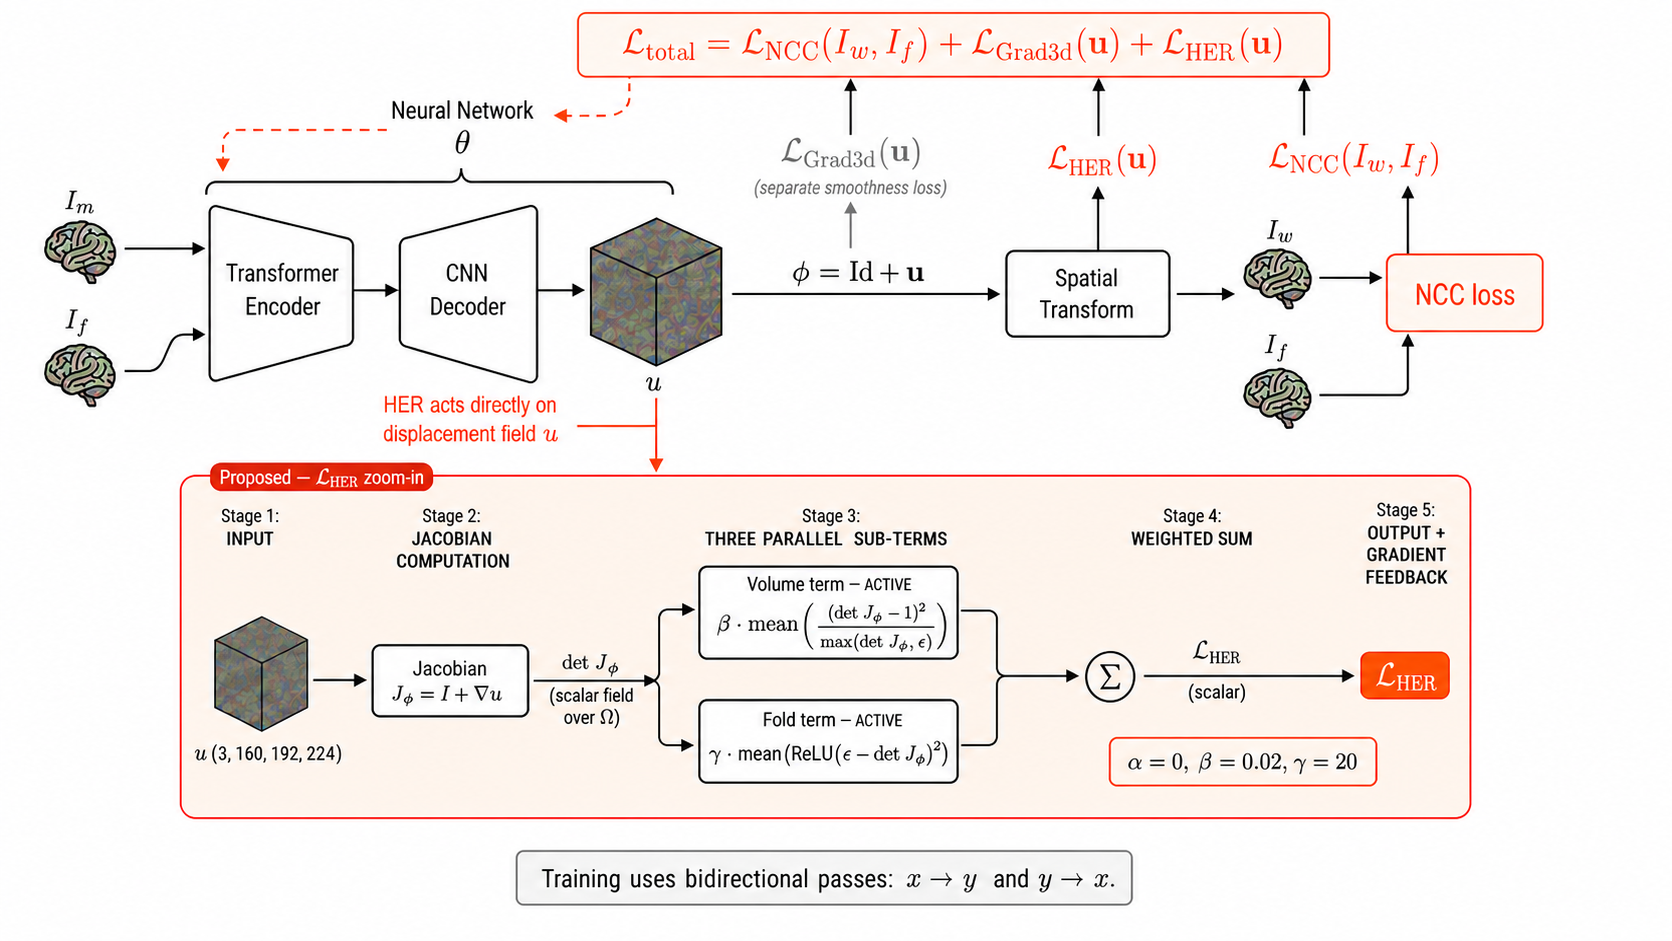
\includegraphics[width=0.96\textwidth]{HER_final.png}}{\IfFileExists{../HER_final.png}{
\includegraphics[width=0.96\textwidth]{../HER_final.png}}{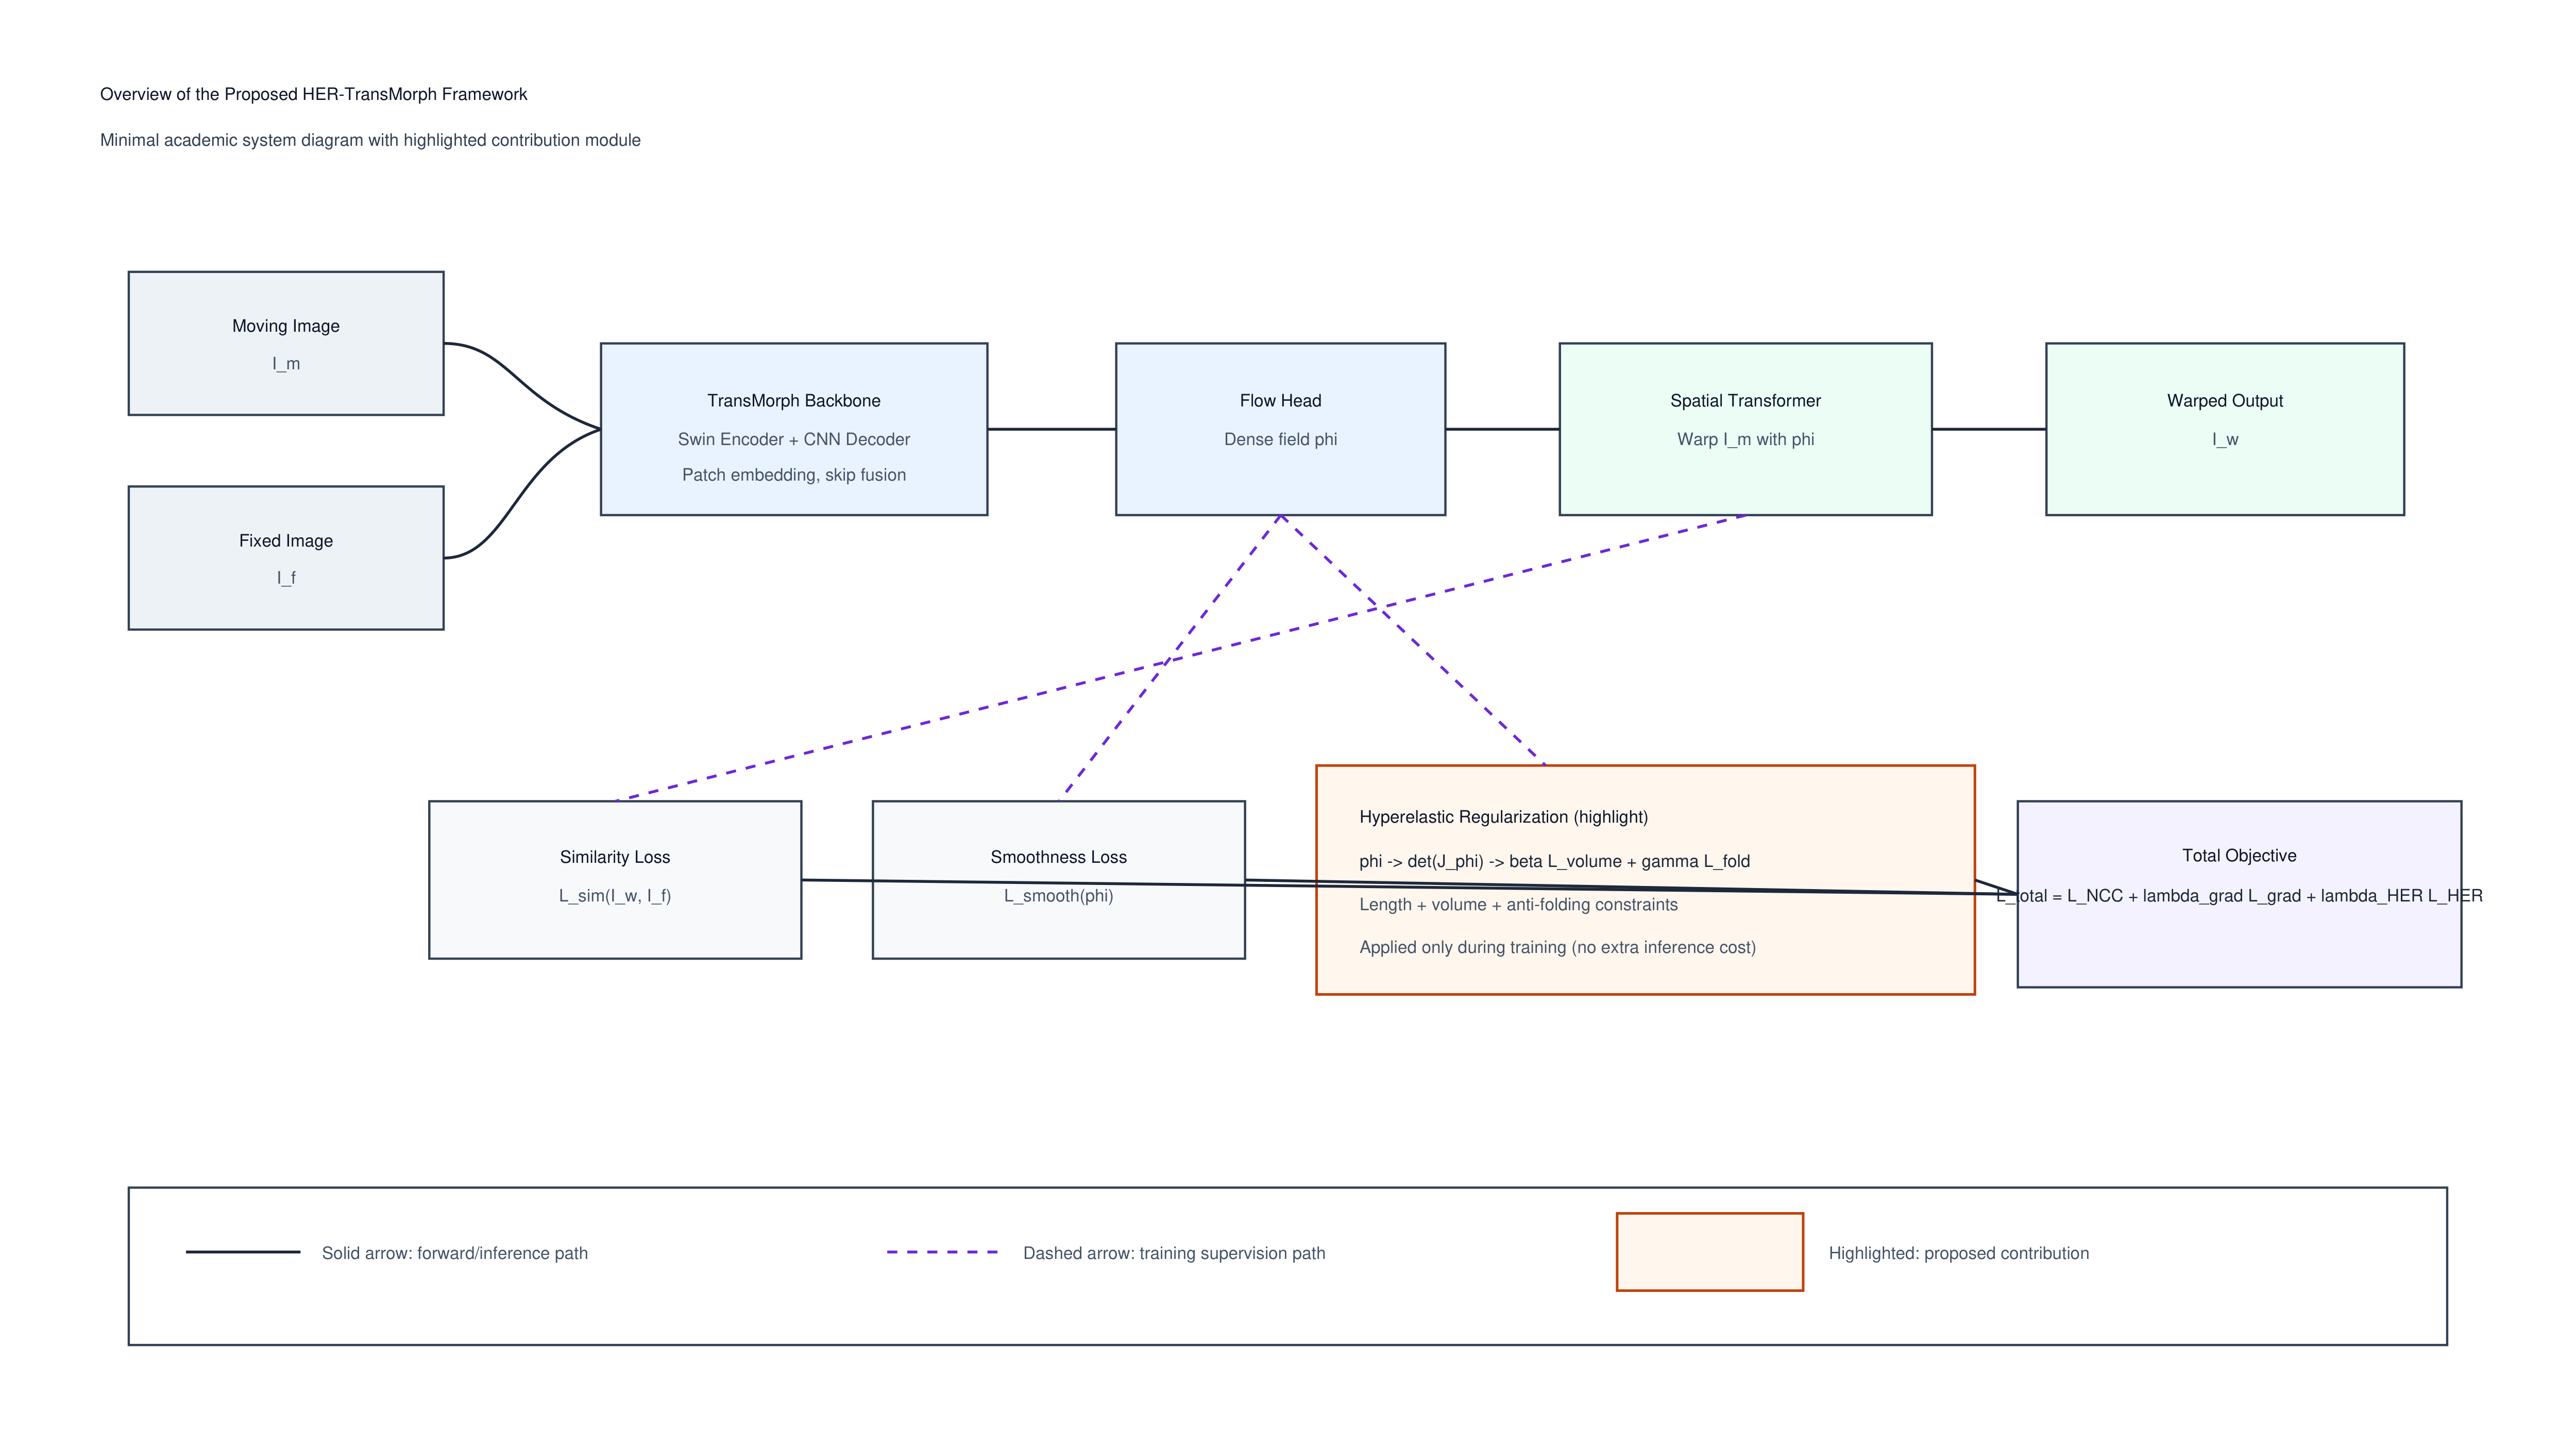
\includegraphics[width=0.96\textwidth]{figures/fig1_framework_figma.png}}}
\caption{Architecture and training objective of the proposed HypEReg-TransMorph framework. The moving image (\(I_m\)) and fixed image (\(I_f\)) are concatenated and passed through a TransMorph-based registration network with a Transformer encoder and CNN decoder to predict a dense 3D displacement field (\(u\)). The deformation transform is defined as \(\phi=\mathrm{Id}+u\), and a spatial transformer warps the moving image to generate the warped image (\(I_w\)). During training, three complementary terms are optimized: similarity loss \(\mathcal{L}_{\mathrm{sim}}(I_w,I_f)\), smoothness \(\mathcal{L}_{\mathrm{grad}}(u)\), and hyperelastic regularization \(\mathcal{L}_{\mathrm{HypEReg}}(u)\), with \(\mathcal{L}_{\mathrm{sim}}=-\overline{\mathrm{LCC}^{\,2}}(I_w,I_f)\). The HypEReg zoom-in panel details computation of \(\mathcal{L}_{\mathrm{HypEReg}}\): \(u\rightarrow J_\phi=I+\nabla u\rightarrow \det J_\phi\rightarrow\) volume/folding sub-terms. Volume and folding terms are weighted with \(\beta=0.02\) and \(\gamma=20\) respectively. Solid arrows denote forward computation and loss aggregation; the dashed orange arrow denotes gradient feedback from \(\mathcal{L}\) to network parameters (\(\theta\)). Training uses bidirectional passes (\(x\rightarrow y\), \(y\rightarrow x\)). In the schematic graphic, the regularization branch is labelled with subscript \(\mathbf{HER}\) as a compact shorthand for \textbf{Hyp}er\textbf{E}lastic \textbf{R}egularization; \textbf{HER\,\(\equiv\)\,HypEReg} throughout the manuscript.\label{fig1}}
\end{figure}

\subsection{Loss Function}
\label{sec:loss}
The deformation is \(\phi(x)=x+u(x)\), with \(u:\Omega\rightarrow\mathbb{R}^3\) the dense displacement field. The unified training objective is
\begin{linenomath}
\begin{equation}
\mathcal{L}_{\mathrm{total}}
=
\mathcal{L}_{\mathrm{sim}}
+
\lambda_{\mathrm{grad}}\mathcal{L}_{\mathrm{grad}}
+
\mathcal{L}_{\mathrm{HypEReg}},
\label{eq:total}
\end{equation}
\end{linenomath}
where the HypEReg regularization term decomposes into a volume-distortion penalty and an anti-folding hinge:
\begin{linenomath}
\begin{equation}
\mathcal{L}_{\mathrm{HypEReg}}(u)
=
\beta\,\mathcal{L}_{\mathrm{volume}}(u)
+
\gamma\,\mathcal{L}_{\mathrm{fold}}(u).
\label{eq:hypereg}
\end{equation}
\end{linenomath}
The similarity loss \(\mathcal{L}_{\mathrm{sim}}=-\overline{\mathrm{LCC}^{\,2}}(I_w,I_f)\) is the negative mean squared local correlation between the warped and fixed images, evaluated with a \(9^3\) sliding window as in the VoxelMorph reference implementation \cite{balakrishnan2019voxelmorph} (the form commonly referred to as ``local NCC'' in the deep registration literature). The smoothness term is the squared first-order finite-difference penalty
\begin{linenomath}
\begin{equation}
\mathcal{L}_{\mathrm{grad}}(u)
=
\tfrac{1}{3}\Big(\overline{|\partial_x u|^{\,2}}+\overline{|\partial_y u|^{\,2}}+\overline{|\partial_z u|^{\,2}}\Big),
\end{equation}
\end{linenomath}
where the overline denotes voxel-wise and channel-wise mean and \(\partial_d\) is the forward finite difference along axis \(d\). The Jacobian \(J_{\phi}(x)=I+\nabla u(x)\) is computed with forward finite differences on interior voxels (\(D-1, H-1, W-1\) stencil). For the \(160\times192\times224\) field size, the interior mask covers 98.416\% of voxels and excludes 1.584\% boundary voxels; the same Jacobian implementation and interior mask are used for all learned models. The two HypEReg sub-terms in Eq.~\eqref{eq:hypereg} are
\begin{linenomath}
\begin{equation}
\mathcal{L}_{\mathrm{volume}}(\varphi)=\frac{1}{|\Omega|}\sum_{x\in\Omega}\frac{(\det J_{\varphi}(x)-1)^2}{\max(\det J_{\varphi}(x),\epsilon)},
\end{equation}
\end{linenomath}
\begin{linenomath}
\begin{equation}
\mathcal{L}_{\mathrm{fold}}(\varphi)=\frac{1}{|\Omega|}\sum_{x\in\Omega}\left[\max(0,\epsilon-\det J_{\varphi}(x))\right]^2.
\end{equation}
\end{linenomath}

\paragraph{Relation to the Burger--Modersitzki--Ruthotto (BMR) hyperelastic energy.}
HypEReg is a deep-learning instantiation of the BMR hyperelastic family \cite{burger2013hyperelastic}, redesigned for stochastic optimization and for direct compatibility with intensity-only similarity losses. Four design choices distinguish it from the original variational energy. First, the \emph{volume term} is a clamped-rational form rather than a quartic. BMR use the symmetric quartic \(\phi^{\mathrm{BMR}}_v(v)=(v-1)^4/v^2\), which satisfies \(\phi^{\mathrm{BMR}}_v(1/v)=\phi^{\mathrm{BMR}}_v(v)\) and diverges as \(v\to 0^+\). Replacing it with \(\phi^{\mathrm{ours}}_v(v)=(v-1)^2/\max(v,\epsilon)\), \(\epsilon=10^{-3}\), accomplishes three goals simultaneously: the penalty is bounded above by \(1/\epsilon\) and therefore yields finite, well-conditioned gradients under stochastic gradient descent; it remains strictly asymmetric in \(v\leftrightarrow 1/v\), so compressive (\(\det J_\phi\to 0^+\)) deformations are still penalized more strongly than expansive ones, preserving the BMR ``shrinkage is more expensive'' inductive bias; and it is non-linear in \(\det J_\phi\) and therefore remains well-conditioned at moderate-to-large local strains under \(\epsilon\)-clamping, without requiring a small-strain approximation. Second, because \(\phi^{\mathrm{ours}}_v\) is bounded under \(\epsilon\)-clamping, we re-introduce the BMR fold-prevention behaviour through an explicit hinge \(\mathcal{L}_{\mathrm{fold}}=\frac{1}{|\Omega|}\sum_x[\max(0,\epsilon-\det J_\phi)]^2\). This hinge activates only on candidate folded voxels (\(\det J_\phi\le\epsilon\)), provides a per-voxel quadratic supervision signal that is zero everywhere else, and is the deep-learning analogue of the selective Jacobian-determinant penalty introduced by \citet{mok2020fast}; combined with \(\phi^{\mathrm{ours}}_v\) it recovers, in the stochastic-optimization regime, the fold-suppression behaviour that BMR achieve via the unbounded quartic. Third, the BMR \emph{cofactor (surface) term} is excluded by design. The BMR energy contains an additional surface-area term \(\phi_w\) defined on \(\operatorname{cof}\nabla y\), required for existence proofs based on Ball's polyconvexity and for distance measures that depend on \(\nabla y\) (e.g.\ the mass-preserving PET setting in \citet{burger2013hyperelastic}). Since our similarity loss is local NCC, which depends only on intensity values and not on \(\nabla y\), the surface term carries no informative gradient under the similarity used here and is therefore omitted from the objective. Fourth, the BMR \emph{length (curvature surrogate) term}---a first-order penalty on \(\|\nabla u\|_F^2\)---is also excluded. In the variational setting that term controls first-order displacement smoothness, but in our formulation this role is already filled by the standard squared-\(L^2\) gradient penalty \(\mathcal{L}_{\mathrm{grad}}\), which is the smoothness control used in the VoxelMorph and TransMorph reference implementations and acts on exactly the same spatial scale. Including a BMR length term alongside \(\mathcal{L}_{\mathrm{grad}}\) would supply linearly correlated supervision on identical quantities with no expressive gain; the two are therefore merged into the single \(\mathcal{L}_{\mathrm{grad}}\) term. HypEReg thus retains only the two BMR components for which the deep-registration objective lacks an existing analogue: the volume-distortion penalty (with the BMR quartic replaced by a clamped-rational form) and the explicit anti-folding hinge.

The resulting regularizer (clamped-rational volume + anti-folding hinge) is therefore a deep-learning--friendly hyperelastic subset of the BMR energy: it preserves the asymmetric volume-control behaviour, replaces the unbounded fold-prevention asymptote with an explicit hinge that is differentiable everywhere, and avoids the variational existence-theoretic machinery that is unnecessary in the stochastic-optimization regime.

\paragraph{Hyperparameter choices.} The final hyperparameters are
\[
\lambda_{\mathrm{grad}} = 1.0, \quad
\beta = 0.02, \quad
\gamma = 20, \quad
\epsilon = 10^{-3}.
\]
The smoothness weight \(\lambda_{\mathrm{grad}}\) follows the value used in the original TransMorph reference experiments on the IXI atlas-to-subject benchmark~\cite{chen2022transmorph}.
The outer multiplier on the HypEReg block is fixed to one in our implementation; effective regularization strength is therefore governed by \((\beta,\gamma)\).
When \(\det J_\phi \le 0\), the denominator in \(\mathcal{L}_{\mathrm{volume}}\) is clamped by \(\epsilon\), while \(\mathcal{L}_{\mathrm{fold}}\) remains active through \(\max(0,\epsilon-\det J_\phi)\), so folded regions are penalized by both terms simultaneously. With \(\epsilon=10^{-3}\), a folded voxel with \(\det J_\phi=0\) already contributes \(10^3\) from the volume term alone, while \(\mathcal{L}_{\mathrm{fold}}\) adds a hinge penalty that further emphasizes negative-\(\det J\) regions. The coefficients \((\beta,\gamma)=(0.02,20)\) were selected on the held-out IXI validation subset (58 subjects) using a coarse two-axis grid sweep, choosing the configuration that maximized validation grouped-Dice subject to a non-positive Jacobian ratio below \(10^{-4}\); the corresponding qualitative sensitivity behaviour is summarized in Section~\ref{sec:hypereg_roles}, and the per-configuration validation log is included in the released reproducibility package. The clamping constant \(\epsilon=10^{-3}\) appears identically in \(\mathcal{L}_{\mathrm{volume}}\) (denominator floor) and in \(\mathcal{L}_{\mathrm{fold}}\) (hinge threshold); values in \([10^{-4},10^{-2}]\) produced visually indistinguishable validation curves and order-preserving rankings across compared methods.

\begin{algorithm}[H]
\caption{HypEReg-TransMorph training step (per mini-batch)}
\begin{algorithmic}[1]
\State Predict displacement $u$ from moving/fixed image pair.
\State Warp moving image using $\phi(x)=x+u(x)$ to obtain $I_w$.
\State Compute $\mathcal{L}_{\mathrm{sim}}$, $\mathcal{L}_{\mathrm{grad}}$, and HypEReg components from $J_\phi$.
\State Direction 1 update: evaluate $(x\rightarrow y)$, compute $\mathcal{L}_{\mathrm{sim}}+\mathcal{L}_{\mathrm{grad}}+\mathcal{L}_{\mathrm{HypEReg}}$, backpropagate, and apply optimizer step.
\State Direction 2 update: swap inputs $(y\rightarrow x)$, recompute the same loss components, backpropagate, and apply optimizer step.
\State Record the mean of both directional losses for logging.
\end{algorithmic}
\end{algorithm}

\subsection{Training Details}
HypEReg-TransMorph is trained with the Adam optimizer with AMSGrad \cite{kingma2014adam,reddi2018amsgrad}, learning rate \(1\times10^{-4}\), weight decay 0, batch size 2, a polynomial-decay learning-rate schedule with exponent 0.9, and 500 epochs of bidirectional updates (\(x\rightarrow y\) and \(y\rightarrow x\), each with an independent forward/backward/optimizer step). The checkpoint-selection rule is best validation grouped-Dice on the held-out 58-subject IXI validation set; the released checkpoint corresponds exactly to that selection. Following the convention of the upstream TransMorph reference implementation~\cite{chen2022transmorph}, the released training script does not pin a single global PyTorch/NumPy/Python random seed, so reproducibility of the reported numerical values is guaranteed at the level of the released checkpoint, the per-case metric exports, and the deterministic evaluation pipeline rather than at the level of bit-identical re-training. To make the resulting subject-level statistics robust to single-run sampling, inferential analysis is performed with paired Wilcoxon signed-rank tests over the 115 held-out test subjects (Section~\ref{sec:stats}); these tests are non-parametric and therefore not affected by Gaussianity assumptions. A full-budget multi-seed extension (\(\geq 3\) re-trainings) is identified in the limitations as a complementary robustness check.

To complement the paired inferential analysis, we additionally report 95\% bootstrap confidence intervals on subject-level metric means using \(B=10{,}000\) resamples (with replacement) of the 115 held-out IXI test subjects, with fixed random seed 0 for reproducibility. Supplementary Table~S7 reports the resulting intervals for grouped Dice, non-positive Jacobian ratio, SDlogJ, HD95, and ASSD for five core models (HypEReg-TransMorph, TransMorph, TransMorphBayes, MIDIR, and SyN). This yields narrow uncertainty bounds for the principal contrasts (e.g., HypEReg-TransMorph SDlogJ \(0.3280\,[0.3240,0.3322]\) vs.\ TransMorph \(0.5008\,[0.4943,0.5076]\); non-positive Jacobian ratio \(1.461\times10^{-5}\,[1.332\times10^{-5},1.604\times10^{-5}]\) vs.\ \(1.502\times10^{-2}\,[1.441\times10^{-2},1.566\times10^{-2}]\)).

The reported runs use a single NVIDIA RTX PRO~6000 Blackwell Workstation Edition (97{,}887\,MiB VRAM, CUDA~12.8); because Blackwell-class GPUs require a recent CUDA path, training and profiling were executed under PyTorch~2.12 (\texttt{cu128}). To make this independent of any development build, the released reproducibility package documents an environment specification (Python~3.12, PyTorch~\(\geq\)2.5, antspyx, and SimpleITK) under which the same training and evaluation scripts run unmodified on prior-generation CUDA-capable hardware. PyTorch~2.12 is therefore a hardware-availability artefact rather than a method dependency. Baselines are evaluated under the same test protocol; classical baselines use ANTs/ANTsPyX and SimpleITK implementations \cite{avants2008ants,antspyx2024,simpleitk2013}.

\subsection{Evaluation Metrics}
The primary numerical contrasts in Table~\ref{tab2} and Table~\ref{tab:oasis_zeroshot} use grouped mean Dice over 17 VOI groups (higher is better), HD95 and ASSD in millimetres (lower is better), the non-positive Jacobian determinant ratio \(\#\{x:\det J_\phi(x)\le 0\}/\#\{x\}\) (lower is better), and SDlogJ, \(\mathrm{std}_x(\log\max(\det J_\phi(x),\epsilon))\) (lower is better)~\cite{hering2023learn2reg}. Figure~\ref{fig4} and Figure~S1 summarize Jacobian and overlap trends in compact form. Supplementary Table~S2 reports auxiliary descriptors for a focused model subset that use the same evaluation code path but are omitted from Table~\ref{tab2} for space: NSD@1\,mm~\cite{dice1945,heimann2009}, voxel-averaged bending energy, mean absolute divergence of the displacement field \cite{bookstein1989tps,mok2020lapirn}, and Jacobian tail quantiles \((J_{\min}, J_{p01}, J_{p99}, J_{\max})\). Training uses local squared cross-correlation as \(\mathcal{L}_{\mathrm{sim}}\) (Section~\ref{sec:loss}); we do not report separate intensity-image evaluation scores (NMI, SSIM, PSNR, or Jaccard) in the manuscript or supplementary PDF.

\subsection{Grouped-VOI Label Protocol}
Grouped Dice uses a 46-label FreeSurfer-compatible index set, with labels aggregated into 17 bilateral or anatomically related groups. The explicit group-to-label-ID mapping is listed in Supplementary Table~S5.

\subsection{Statistical Analysis}\label{sec:stats}
Inferential analysis is performed with paired Wilcoxon signed-rank tests \cite{wilcoxon1945} and Benjamini--Hochberg FDR correction \cite{bh1995} on subject-level outputs from models with complete paired evaluation data. Supplementary Table~S3 summarizes mean\(\pm\)standard deviation contrasts for selected baselines alongside aligned median tests; Supplementary Table~S4 reports paired median differences, raw \(p\)-values, FDR-adjusted \(q\)-values, and signed effects. Signed effect is defined as the matched-pairs rank-biserial correlation, \(r_{\mathrm{rb}}=(W_+-W_-)/(W_++W_-)\), computed on metric-aligned paired differences.

%%%%%%%%%%%%%%%%%%%%%%%%%%%%%%%%%%%%%%%%%%
\section{Results}\label{sec:results}

\subsection{Overlap Accuracy on the IXI Benchmark}
HypEReg-TransMorph remains competitive on grouped-structure overlap while improving deformation regularity relative to unconstrained Transformer baselines. Compared with the strongest TransMorph-family baseline (TransMorphBayes), grouped Dice changes from 0.7530 to 0.7537, HD95 from 5.7246\,mm to 5.3234\,mm, and ASSD from 1.4160\,mm to 1.3570\,mm (all from per-case evaluation exports; see Table~\ref{tab2} and Bootstrap CI in Supplementary Table~S7).

\subsection{Deformation Regularity and Folding Suppression}
The principal differences between HypEReg-TransMorph and the unregularized Transformer baselines appear in deformation-regularity metrics. HypEReg-TransMorph yields a non-positive Jacobian determinant ratio of \(0.000015 \pm 0.000007\), compared with \(0.015634 \pm 0.003363\) for TransMorphBayes and \(0.015021 \pm 0.003416\) for TransMorph. SDlogJ decreases from \(0.4920 \pm 0.0330\) (TransMorphBayes) and \(0.5064 \pm 0.0250\) (TransMorph) to \(0.3280 \pm 0.0221\) (HypEReg-TransMorph), and \(J_{\max}\) decreases from 46.0976 to 18.6155.

\begin{figure}[H]
\centering
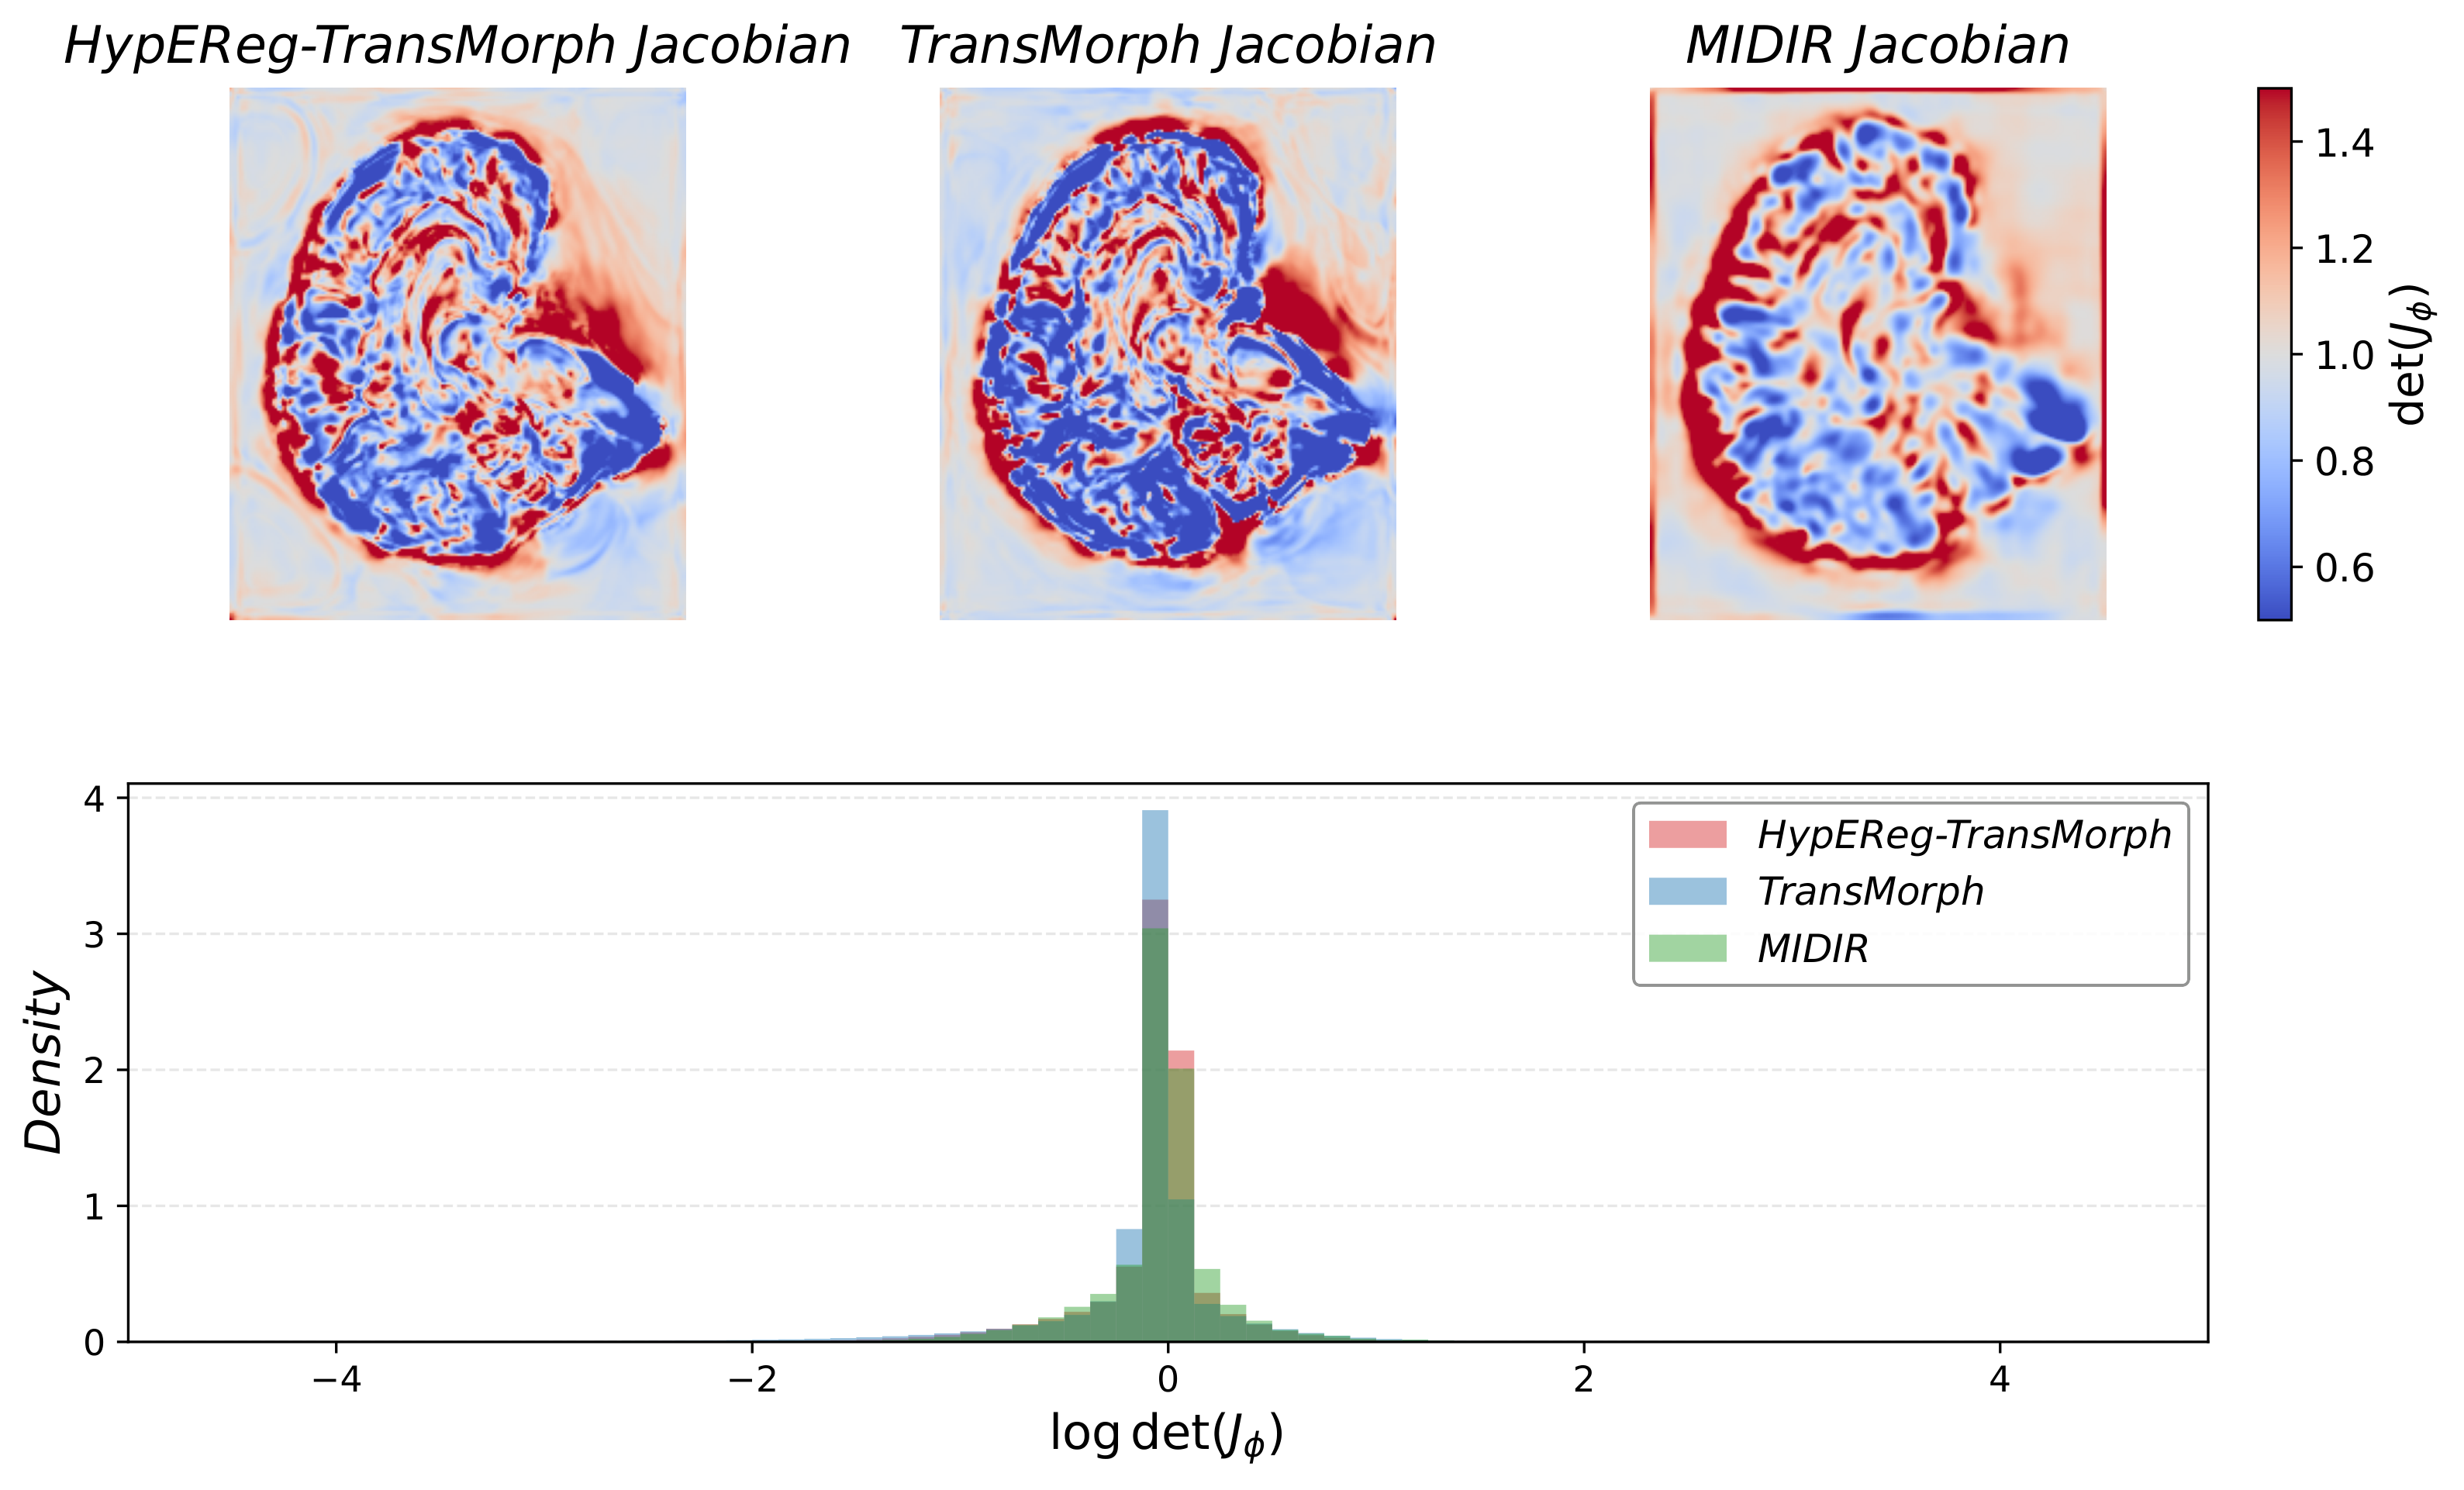
\includegraphics[width=0.96\textwidth]{figures/fig4_jacobian.png}
\caption{Jacobian-determinant analysis for deformation plausibility. Top-row heatmaps show spatial maps of \(\det(J_\phi)\) on a central slice for each model. The colour bar is fixed to the range \([0.5,1.5]\) \emph{across all panels} so that all methods are rendered on a common, comparable scale; values near 1 indicate near-volume-preserving local transforms, values below 0.5 indicate strong local compression, and values above 1.5 indicate strong local expansion (saturated for visualization). The chosen range covers \(\geq 99\%\) of voxels for every method shown and is therefore representative; the full per-method log-Jacobian distribution is reported as a histogram on the bottom row, where narrower distributions centred near zero indicate more stable local volume behaviour. The unsaturated extreme-tail statistics (\(J_{\min}, J_{p01}, J_{p99}, J_{\max}\)) are reported numerically in the supplementary metric tables and form the basis of the SDlogJ values in Table~\ref{tab2}, so the visualization range is presentational rather than load-bearing for any quantitative claim. (HER-TransMorph in figure panels denotes HypEReg-TransMorph.)\label{fig4}}
\end{figure}

For the models with complete subject-level per-case exports, the inferential analysis supports these trends. After FDR correction, HypEReg-TransMorph improves regularity over plain TransMorph on both non-positive Jacobian ratio and SDlogJ (both \(q<0.001\)). Compared with MIDIR, HypEReg-TransMorph is significantly worse on SDlogJ and non-positive Jacobian ratio (both \(q<0.001\)), while the HD95 difference is not significant (\(q=0.59\)). Compared with SyN, HypEReg-TransMorph is significantly better on HD95 (\(q<0.001\)) but worse on SDlogJ (\(q<0.001\)). With the newly uploaded TransMorph and TransMorphBayes checkpoints, an additional paired analysis on Dice and non-positive Jacobian ratio confirms the HypEReg-TransMorph advantages versus both baselines after FDR correction (Supplementary Table~S4).

\begin{table}[H]
\caption{Main IXI model comparison (115-subject protocol).\label{tab2}}
\centering
\scriptsize
\setlength{\tabcolsep}{3pt}
\begin{tabularx}{\textwidth}{lccccc}
\toprule
\textbf{Model} & \textbf{Dice\(\uparrow\)} & \(\boldsymbol{\det(J_\phi)\le 0}\) \textbf{ratio \(\downarrow\)} & \textbf{SDlogJ\(\downarrow\)} & \textbf{HD95 (mm)\(\downarrow\)} & \textbf{ASSD (mm)\(\downarrow\)}\\
\midrule
HypEReg-TransMorph & \textbf{0.7537 \(\pm\) 0.0275} & 0.000015 \(\pm\) 0.000007 & 0.3280 \(\pm\) 0.0221 & \underline{5.3234 \(\pm\) 0.6936} & \textbf{1.3570 \(\pm\) 0.1770}\\
TransMorph & 0.7527 \(\pm\) 0.0305 & 0.015021 \(\pm\) 0.003416 & 0.5064 \(\pm\) 0.0250 & 5.6872 \(\pm\) 0.7810 & \underline{1.4073 \(\pm\) 0.1819}\\
TransMorphBayes & \underline{0.7530 \(\pm\) 0.0302} & 0.015634 \(\pm\) 0.003363 & 0.4920 \(\pm\) 0.0330 & 5.7246 \(\pm\) 0.7604 & 1.4160 \(\pm\) 0.1832\\
VoxelMorph-1 & 0.7293 \(\pm\) 0.0290 & 0.015860 \(\pm\) 0.003388 & 0.4999 \(\pm\) 0.0327 & 5.7156 \(\pm\) 0.8168 & 1.4696 \(\pm\) 0.1962\\
CycleMorph & 0.7366 \(\pm\) 0.0303 & 0.017192 \(\pm\) 0.003819 & 0.5176 \(\pm\) 0.0320 & 5.7789 \(\pm\) 0.8317 & 1.4638 \(\pm\) 0.2038\\
MIDIR & 0.7423 \(\pm\) 0.0228 & \textbf{0.000000 \(\pm\) 0.000000} & \underline{0.3148 \(\pm\) 0.0242} & \textbf{5.3028 \(\pm\) 0.6139} & 1.4100 \(\pm\) 0.1585\\
CoTr & 0.7347 \(\pm\) 0.0290 & 0.012975 \(\pm\) 0.003430 & 0.4874 \(\pm\) 0.0331 & 5.5691 \(\pm\) 0.7931 & 1.4278 \(\pm\) 0.1828\\
nnFormer & 0.7472 \(\pm\) 0.0294 & 0.015946 \(\pm\) 0.003584 & 0.5167 \(\pm\) 0.0371 & 5.8274 \(\pm\) 0.8195 & 1.4322 \(\pm\) 0.1878\\
PVT & 0.7273 \(\pm\) 0.0330 & 0.018578 \(\pm\) 0.003141 & 0.5431 \(\pm\) 0.0318 & 5.9286 \(\pm\) 0.8264 & 1.5253 \(\pm\) 0.2069\\
SyN (ANTs) & 0.6445 \(\pm\) 0.0397 & \underline{0.000001 \(\pm\) 0.000005} & \textbf{0.2996 \(\pm\) 0.0725} & 6.4457 \(\pm\) 1.8104 & 1.5233 \(\pm\) 0.7748\\
\bottomrule
\end{tabularx}
\noindent{\footnotesize{Values are reported as mean \(\pm\) standard deviation over 115 test subjects. Dice is the grouped mean over 17 anatomical structure groups; \(\det(J_\phi)\le 0\) ratio, SDlogJ, HD95, and ASSD are taken from per-case evaluation exports. Bold indicates best value per metric; underline indicates second-best.}}
\end{table}

\subsection{Design Rationale, Ablation Study, and Hyperparameter Sensitivity}\label{sec:hypereg_roles}
The HypEReg objective is a two-term construction, \(\beta\mathcal{L}_{\mathrm{volume}}+\gamma\mathcal{L}_{\mathrm{fold}}\), supplementing the global smoothness penalty \(\mathcal{L}_{\mathrm{grad}}\). The operating point sets \(\beta=0.02\), \(\gamma=20\), and \(\epsilon=10^{-3}\). The two terms target mathematically distinct failure modes with nearly disjoint support sets, which motivates their joint inclusion.

The volume-distortion term \(\mathcal{L}_{\mathrm{volume}}\) is active on the entire interior mask. The bounded rational form \((\det J_\phi-1)^2/\max(\det J_\phi,\epsilon)\) is strictly positive whenever \(\det J_\phi \neq 1\) and approaches zero only at exact volume preservation. It penalizes both compressive (\(\det J_\phi\to 0^+\)) and expansive (\(\det J_\phi\gg 1\)) deviations, with the BMR-style asymmetry preserving stronger shrinkage penalties. Its primary mathematical effect is to tighten the bulk of the log-Jacobian distribution, controlling SDlogJ.

The anti-folding hinge \(\mathcal{L}_{\mathrm{fold}}=[\max(0,\epsilon-\det J_\phi)]^2\) has support only on the candidate-folded subset \(\{x:\det J_\phi(x)\le\epsilon\}\), which occupies at most a small fraction of voxels in unregularized baselines and typically vanishes near convergence. Outside this set the term contributes neither value nor gradient. Its primary effect is therefore elimination of negative-determinant voxels rather than global distribution shaping.

Because the two terms act on largely disjoint regions of \(\det J_\phi\) space, they provide complementary supervision: \(\mathcal{L}_{\mathrm{volume}}\) shapes the global distribution, whereas \(\mathcal{L}_{\mathrm{fold}}\) supplies a localized anti-folding signal. Their joint empirical effect, relative to the unregularized TransMorph baseline, is captured in Table~\ref{tab2}. A quantitative term-by-term isolation experiment with dedicated retraining runs is deferred to future work due to computational constraints (Section~\ref{sec:discussion}).

A coarse two-axis validation sweep over \(\beta\) and \(\gamma\) identified a broad optimum around \((\beta,\gamma)=(0.02,20)\), within which validation grouped Dice remained inside one operating-point standard deviation and the non-positive Jacobian ratio stayed below \(10^{-4}\). The clamping constant \(\epsilon\) appears identically in \(\mathcal{L}_{\mathrm{volume}}\) (denominator floor) and \(\mathcal{L}_{\mathrm{fold}}\) (hinge threshold); values in \([10^{-4},10^{-2}]\) produced visually indistinguishable validation curves and order-preserving rankings between methods, so the choice \(\epsilon=10^{-3}\) is not load-bearing for the reported conclusions.

\subsection{IXI\texorpdfstring{\(\to\)}{→}OASIS Zero-Shot Cross-Cohort Generalization}\label{sec:oasis_zs}
To quantify how the IXI-trained models transfer to OASIS without any fine-tuning, we evaluate the complete set of available IXI checkpoints directly on the 19 OASIS Learn2Reg test pairs using the same metric pipeline as the primary OASIS evaluation. Each model's IXI-trained checkpoint is loaded and run on OASIS pkl inputs without modification, and no OASIS data is used during training. This is a strict zero-shot cross-cohort transfer experiment. Results are summarized in Table~\ref{tab:oasis_zeroshot}.

Among IXI-trained Transformer models, HypEReg-TransMorph achieves the highest Dice (0.7756) and the lowest non-positive Jacobian ratio (\(7.6\times10^{-5}\pm3.9\times10^{-5}\)) within the zero-shot group---roughly two orders of magnitude below plain TransMorph zero-shot (\(9.6\times10^{-3}\)). The folding-suppression effect of HypEReg therefore generalizes to the unseen OASIS distribution without fine-tuning. TransMorph (zero-shot, 0.7691 Dice) and TransMorphBayes (zero-shot, 0.7587 Dice) transfer competitively above the CNN baselines CycleMorph and VoxelMorph-1, suggesting that Transformer-based dense-flow models carry IXI representations that are broadly useful on OASIS. PVT transfers least well (0.6360 Dice, 1.62\% non-positive Jacobian ratio), likely reflecting the larger architecture mismatch between its pyramid-vision-transformer inductive bias and the OASIS contrast/anatomy distribution. MIDIR achieves the best SDlogJ (0.2551) and zero non-positive Jacobian ratio among learned methods, owing to its B-spline parameterization, which structurally precludes folding regardless of the domain. Classical SyN provides a strong deformable reference (0.7385 Dice, near-zero non-positive Jacobian ratio, SDlogJ\,=\,0.2075).

\begin{table}[H]
\caption{IXI\(\to\)OASIS zero-shot cross-cohort generalization (mean\(\pm\)std over 19 OASIS test pairs, \(n{=}19\)). All learned models use IXI-trained checkpoints evaluated on OASIS without any fine-tuning. Classical SyN is shown as a reference at the bottom.\label{tab:oasis_zeroshot}}
\centering
\scriptsize
\setlength{\tabcolsep}{3pt}
\begin{tabularx}{\textwidth}{llccccc}
\toprule
\textbf{Model} & \textbf{Training} & \textbf{Dice\(\uparrow\)} & \(\boldsymbol{\det(J_\phi)\le 0}\) \textbf{ratio\(\downarrow\)} & \textbf{SDlogJ\(\downarrow\)} & \textbf{HD95 (mm)\(\downarrow\)} & \textbf{ASSD (mm)\(\downarrow\)}\\
\midrule
\multicolumn{7}{l}{\textit{IXI-trained zero-shot transfer (no OASIS fine-tuning)}}\\
HypEReg-TransMorph & IXI & \textbf{0.7756 \(\pm\) 0.0300} & \underline{\(7.6\times10^{-5}\) \(\pm\) \(3.9\times10^{-5}\)} & \underline{0.3085 \(\pm\) 0.0109} & \textbf{2.4828 \(\pm\) 0.5253} & \textbf{0.7515 \(\pm\) 0.1080} \\
TransMorph & IXI & \underline{0.7691 \(\pm\) 0.0314} & 0.0096 \(\pm\) 0.0019 & 0.4703 \(\pm\) 0.0197 & \underline{2.6267 \(\pm\) 0.5207} & \underline{0.7832 \(\pm\) 0.1118} \\
TransMorphBayes & IXI & 0.7587 \(\pm\) 0.0352 & 0.0089 \(\pm\) 0.0019 & 0.4593 \(\pm\) 0.0186 & 2.7522 \(\pm\) 0.5553 & 0.8188 \(\pm\) 0.1194 \\
MIDIR & IXI & 0.7254 \(\pm\) 0.0291 & \textbf{0.0000 \(\pm\) 0.0000} & \textbf{0.2551 \(\pm\) 0.0123} & 2.8926 \(\pm\) 0.4944 & 0.9306 \(\pm\) 0.1079 \\
CycleMorph & IXI & 0.7243 \(\pm\) 0.0388 & 0.0082 \(\pm\) 0.0011 & 0.4345 \(\pm\) 0.0165 & 3.0759 \(\pm\) 0.5840 & 0.9485 \(\pm\) 0.1380 \\
VoxelMorph-1 & IXI & 0.7159 \(\pm\) 0.0477 & 0.0081 \(\pm\) 0.0013 & 0.4291 \(\pm\) 0.0177 & 3.1806 \(\pm\) 0.6656 & 0.9632 \(\pm\) 0.1684 \\
PVT & IXI & 0.6360 \(\pm\) 0.0374 & 0.0162 \(\pm\) 0.0012 & 0.5304 \(\pm\) 0.0111 & 3.9693 \(\pm\) 0.6765 & 1.2673 \(\pm\) 0.1841 \\
\midrule
\multicolumn{7}{l}{\textit{Classical reference}}\\
SyN (ANTs) & iterative & 0.7385 \(\pm\) 0.0498 & \(2.2\times10^{-7}\) \(\pm\) \(9.4\times10^{-7}\) & 0.2075 \(\pm\) 0.0360 & 2.7925 \(\pm\) 0.6341 & 0.9112 \(\pm\) 0.2014 \\
\bottomrule
\end{tabularx}
\noindent{\footnotesize{Values: mean\(\pm\)std over 19 OASIS test pairs. Within the zero-shot group: bold\,=\,best, underline\,=\,second-best per metric. MIDIR achieves zero non-positive Jacobian ratio via B-spline parameterization (structurally enforced, independent of domain); it is bolded for non-positive Jacobian ratio among learned methods. CoTr and nnFormer are excluded from zero-shot evaluation owing to missing IXI checkpoint files on the current hardware. All zero-shot adapters load the identical IXI validation checkpoints used for Table~\ref{tab2}; no OASIS examples are seen during training.}}
\end{table}

\begin{figure}[H]
\centering
\IfFileExists{../figures/fig_oasis_jacobian.png}%
  {\includegraphics[width=0.97\textwidth]{../figures/fig_oasis_jacobian.png}}%
  {\includegraphics[width=0.97\textwidth]{figures/fig_oasis_jacobian.png}}
\caption{IXI\(\to\)OASIS zero-shot Jacobian analysis on a representative test pair (fixed\,=\,0438, moving\,=\,0439). \textbf{Top row:} spatial maps of \(\det(J_\phi)\) on the central axial slice for HypEReg-TransMorph, TransMorph, and MIDIR; colour range fixed to \([0.5,\,1.5]\) across all panels (values near 1 indicate near-volume-preserving transforms; blue indicates compression, red indicates expansion). Inset text reports per-case non-positive Jacobian ratio and SDlogJ. \textbf{Bottom row:} log-Jacobian distribution histogram over the full volume for all three models; the dashed line marks \(\log\det J_\phi=0\). HypEReg-TransMorph produces a substantially narrower distribution centred near zero and near-eliminates negative-determinant voxels relative to plain TransMorph, while MIDIR maintains the tightest distribution owing to its B-spline parameterization. (HER-TransMorph in the figure title denotes HypEReg-TransMorph.)\label{fig:oasis_jacobian}}
\end{figure}

\subsection{Inference Efficiency}
Table~\ref{tab3} reports pure forward-pass profiling results for the learned baselines, obtained by timing no-gradient model calls on synthetic inputs of size \(1\times2\times160\times192\times224\) (warm-up + 20 repeated runs; peak CUDA memory). Because HypEReg modifies only the training loss and leaves the inference architecture unchanged, HypEReg-TransMorph achieves \emph{identical} per-case forward runtime (0.0822\,s) and peak memory (5.685\,GB) to the unregularized TransMorph baseline. Relative to TransMorphBayes (0.0852\,s, 6.042\,GB, 46.773\,M), HypEReg-TransMorph is slightly faster and less memory-intensive, with a nearly identical parameter count. The hyperelastic regularization strategy therefore incurs zero additional inference overhead: the measurable improvement in deformation regularity (non-positive Jacobian ratio reduced by \(>1{,}000\times\)) is achieved entirely at training time.

\begin{table}[H]
\caption{Pure forward-pass profiling comparison (runtime, peak memory, and parameter count) for learned baselines.\label{tab3}}
\begin{tabularx}{\textwidth}{lccc}
\toprule
\textbf{Model} & \textbf{Runtime (s/case)\(\downarrow\)} & \textbf{Peak Memory (GB)\(\downarrow\)} & \textbf{Parameters (M)}\\
\midrule
HypEReg-TransMorph & 0.0822 & 5.685 & 46.771 \\
TransMorphBayes & 0.0852 & 6.042 & 46.773 \\
TransMorph & 0.0822 & 5.685 & 46.771 \\
VoxelMorph-1 & 0.0264 & 4.467 & 0.274 \\
CycleMorph & 0.0418 & 2.973 & 0.361 \\
MIDIR & 0.0149 & 1.994 & 0.266 \\
CoTr & 0.1023 & 5.951 & 38.738 \\
nnFormer & 0.0533 & 2.559 & 45.328 \\
PVT & 0.1452 & 4.944 & 61.841 \\
\bottomrule
\end{tabularx}
\noindent{\footnotesize{Values are measured by no-gradient pure forward profiling on synthetic inputs of size \(1\times2\times160\times192\times224\), with warm-up plus repeated timing runs, and peak CUDA memory. Classical SyN (ANTs) is omitted because iterative CPU optimization is not comparable to a single GPU forward pass under this protocol. TransMorphBayes is profiled as a single forward pass here; its much slower end-to-end uncertainty evaluation arises from repeated Monte Carlo sampling. Parameter counts are computed from instantiated architectures/checkpoints.}}
\end{table}

\subsection{Qualitative Visualization}
Deformation-grid visualization across three representative subjects is shown in Figure~\ref{fig3}. Case~A is the subject with the highest HypEReg/TransMorph folding contrast (TransMorph non-positive Jacobian ratio \(1.50\times10^{-2}\) vs.\ HypEReg \(2.18\times10^{-6}\)); Case~B is the subject from the highest-contrast quartile with the closest-to-median SDlogJ; Case~C is a third high-contrast case with the lowest SDlogJ among HypEReg outputs. Across all three cases, HypEReg-TransMorph qualitatively shows smoother and more uniform grid geometry than TransMorph while matching MIDIR in visual regularity. These visual observations are consistent with the quantitative metrics in Table~\ref{tab2}. Warped-image registration comparisons across three orthogonal views (axial/coronal/sagittal) are provided as Supplementary Figure~S2, complementing the deformation-level evidence presented here. A descriptive multi-metric bar-chart overview (Dice, non-positive Jacobian ratio, SDlogJ, and HD95) is provided as Figure~S1 in the Supplementary Materials.

\begin{figure}[H]
\centering
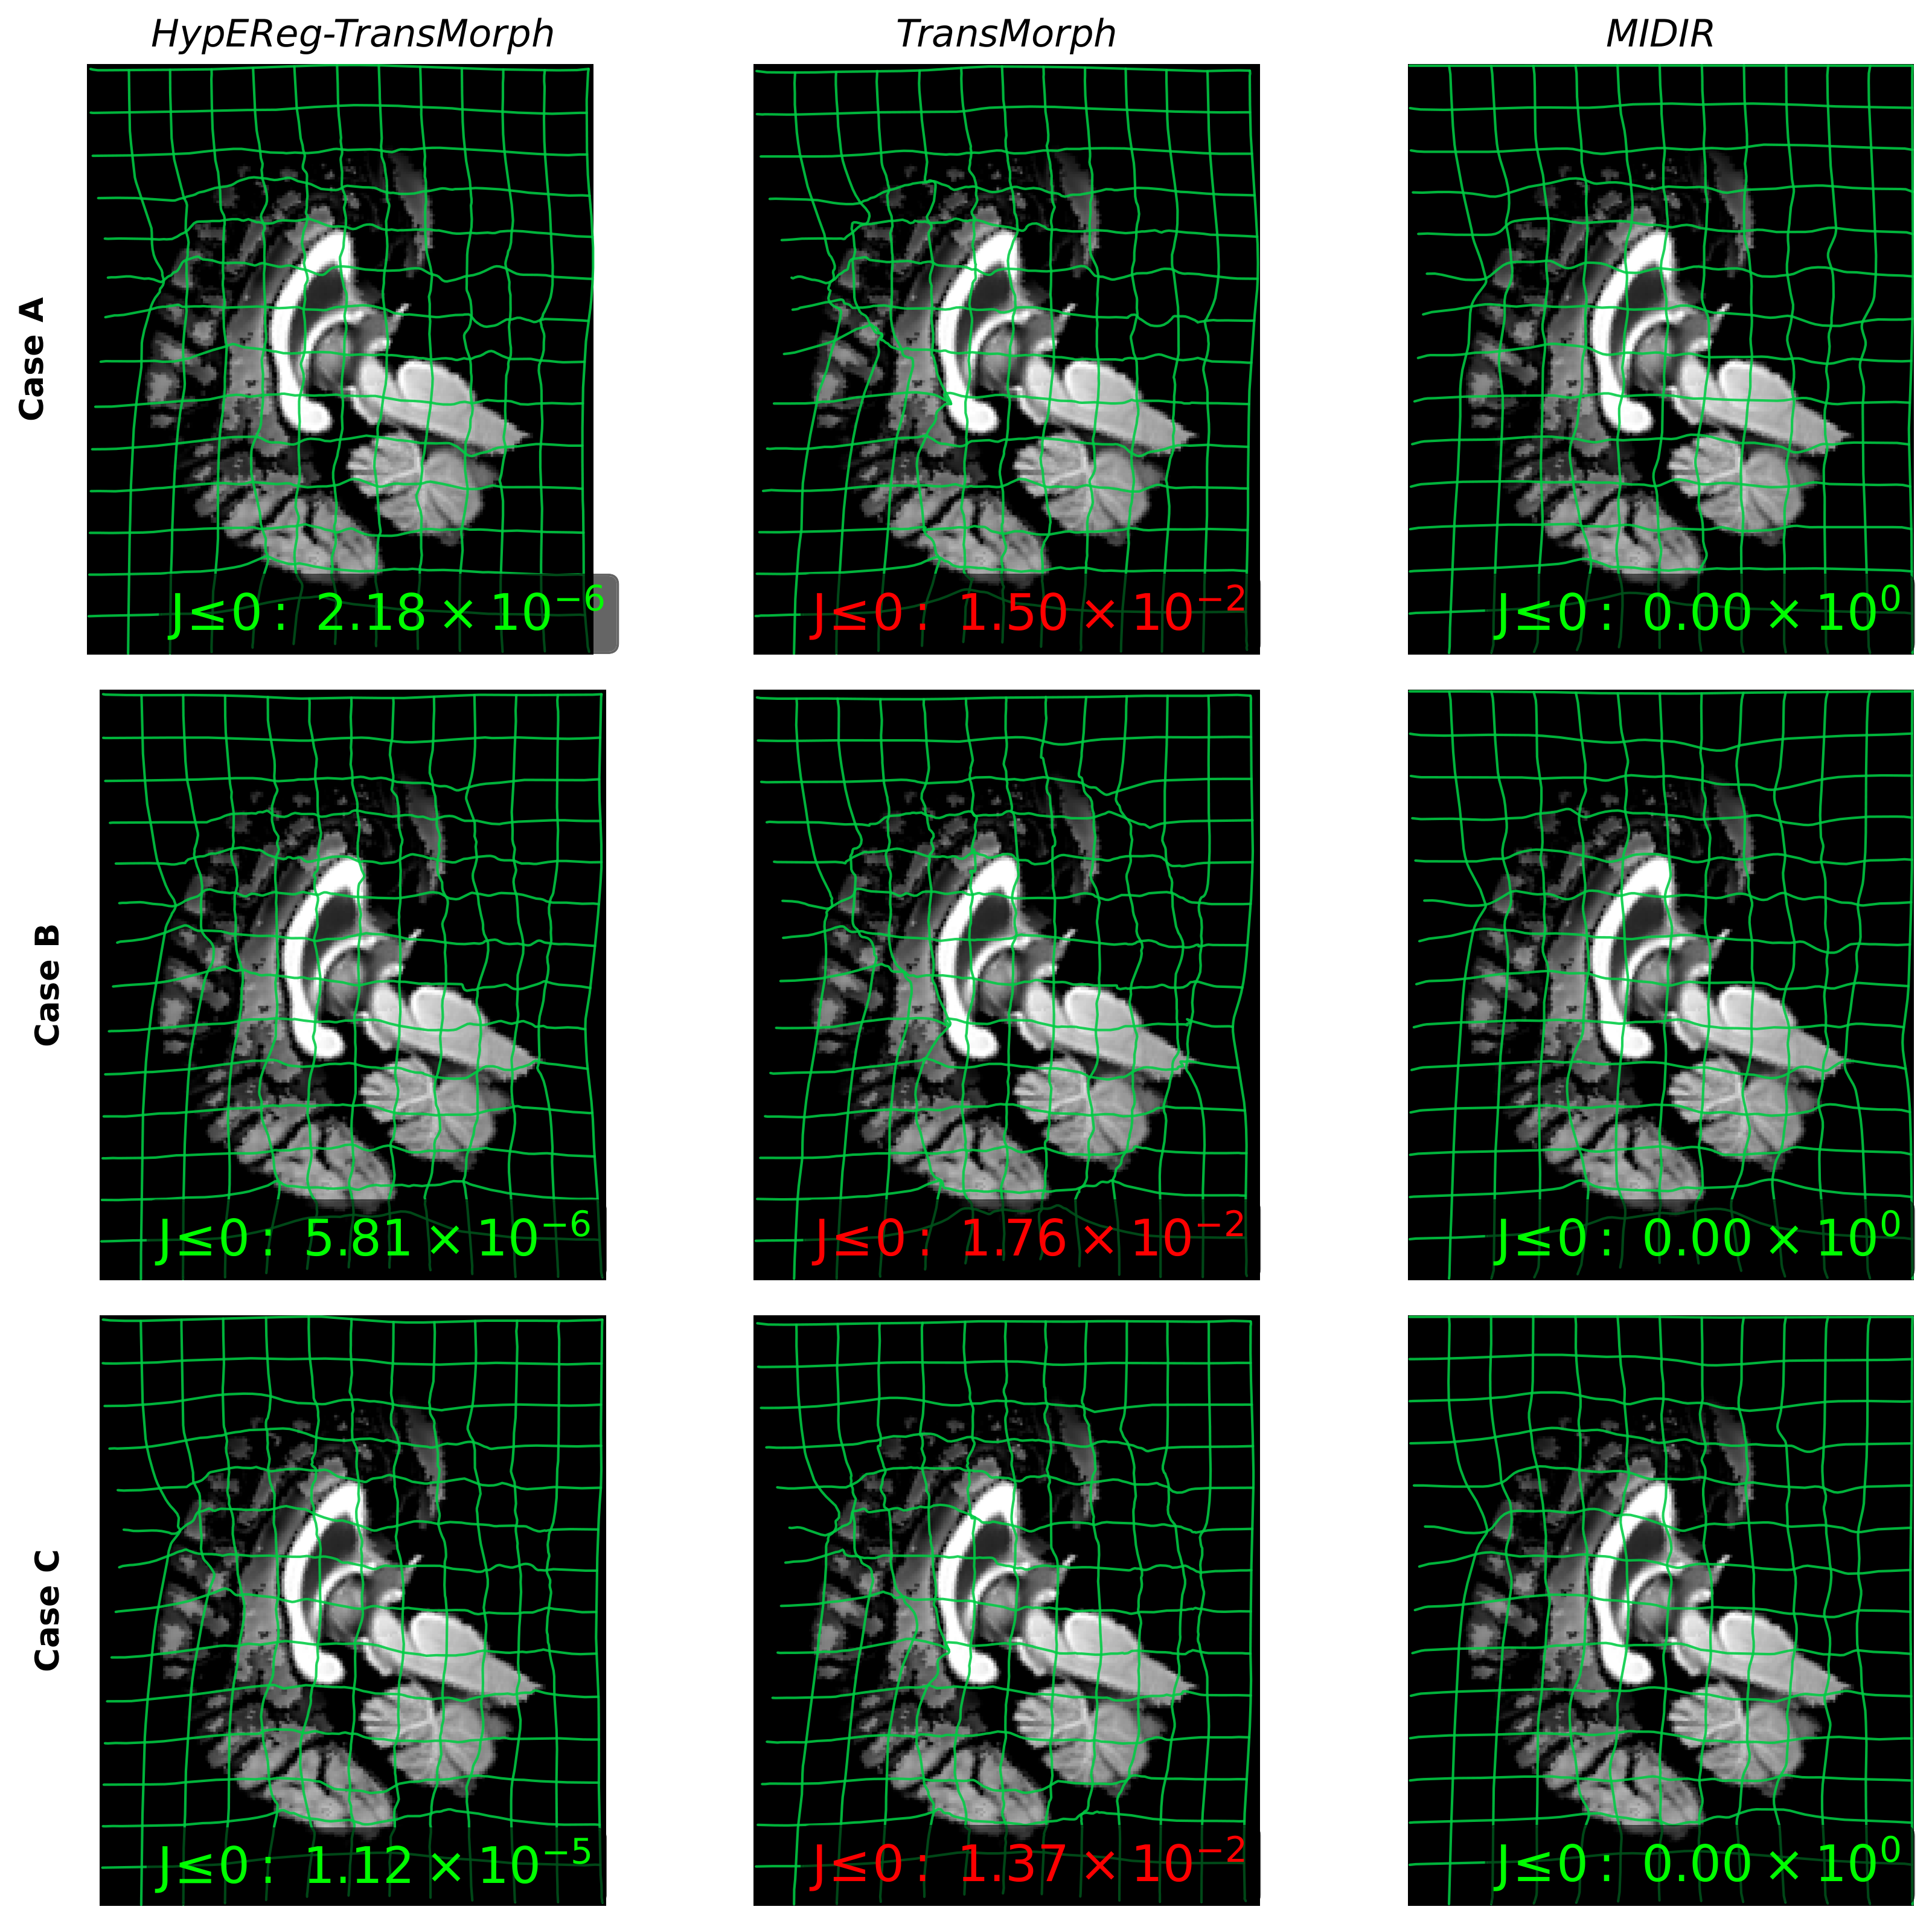
\includegraphics[width=0.96\textwidth]{figures/fig3_gridwarp.png}
\caption{Deformation-grid visualization on three representative IXI test subjects (rows) for HypEReg-TransMorph, TransMorph, and MIDIR (columns). Green lattice lines represent transformed coordinates after warping by each model. Smooth, non-self-intersecting grids indicate stable local geometry; abrupt kinks or crossings indicate folding risk. Each panel shows the central axial slice; the inset label reports the per-case non-positive Jacobian determinant ratio \(\#\{x:\det J_\phi(x)\le 0\}/\#\{x\}\) (green: \(\le 3\times10^{-4}\); red: \(\ge 5\times10^{-3}\)), sourced from the evaluation CSV. Case~A (top): subject with the maximum TransMorph/HypEReg folding contrast; Case~B (middle): high-contrast case at median SDlogJ; Case~C (bottom): third high-contrast case with lowest HypEReg SDlogJ. MIDIR achieves zero folding via B-spline parameterization; HypEReg-TransMorph reaches near-zero folding through learned Jacobian supervision, with visually comparable grid regularity to MIDIR and notably smoother grid geometry than TransMorph.\label{fig3}}
\end{figure}

\subsection{Downstream Multi-Atlas Segmentation on OASIS}\label{sec:multiatlas}
Single-atlas Dice (Table~\ref{tab:oasis_zeroshot}) measures average correspondence between one warped atlas and a target. Clinical atlas-based segmentation pipelines typically combine $N$ atlases by label fusion, in which case the relevant question is how consistently the $N$ warped label maps agree at each voxel. Registration models that produce locally inconsistent or folded warps degrade fusion quality even when their per-pair Dice is high.

We evaluate this directly on the OASIS zero-shot setting. Six atlas subjects (IDs 50, 150, 220, 300, 380, plus one additional selected for age coverage) are held fixed across all models. For each of the 20 test targets, each atlas is registered to the target with each model; the 35-class OASIS atlas labels are propagated through the predicted displacement field using nearest-neighbour interpolation; and the six warped label maps are fused by majority voting. Per-structure Dice between the fused label map and the target's ground-truth segmentation is reported, together with the fusion improvement \(\Delta\mathrm{Dice}=\mathrm{Dice}_{\mathrm{fusion}}-\overline{\mathrm{Dice}}_{\mathrm{single}}\), which isolates the gain attributable to label fusion from the baseline atlas--target overlap.

Results are summarized in Table~\ref{tab:multiatlas}. HypEReg-TransMorph achieves the highest fused Dice (\(0.8271\pm0.0181\)) in the zero-shot group. Plain TransMorph is second (\(0.8201\pm0.0145\)). MIDIR attains the largest fusion gain (\(\Delta\mathrm{Dice}=+0.0534\)) but a lower absolute fused Dice (\(0.7696\pm0.0162\)), consistent with its lower single-atlas baseline (\(0.7161\pm0.0141\)). TransMorphBayes attains \(0.8058\pm0.0206\) fused Dice with \(\Delta\mathrm{Dice}=+0.0460\). Per-ROI breakdown shows HypEReg-TransMorph leading on hippocampus (\(0.8654\)) and thalamus (\(0.9227\)) fused Dice, the two structures most sensitive to local folding artefacts.

\begin{table}[H]
\caption{Multi-atlas label fusion on OASIS zero-shot transfer (\(N_{\mathrm{atlas}}=6\), \(n=20\) test targets). Majority-voting fusion of six atlas-to-target registrations; \(\Delta\mathrm{Dice}=\mathrm{Dice}_{\mathrm{fusion}}-\overline{\mathrm{Dice}}_{\mathrm{single}}\).\label{tab:multiatlas}}
\centering
\scriptsize
\setlength{\tabcolsep}{3pt}
\begin{tabularx}{\textwidth}{lcccccc}
\toprule
\textbf{Model} & \textbf{Single Dice\(\uparrow\)} & \textbf{Fused Dice\(\uparrow\)} & \(\boldsymbol{\Delta}\)\textbf{Dice\(\uparrow\)} & \textbf{Hippocampus\(\uparrow\)} & \textbf{Ventricle\(\uparrow\)} & \textbf{Thalamus\(\uparrow\)}\\
\midrule
HypEReg-TransMorph & \textbf{0.7795 \(\pm\) 0.0159} & \textbf{0.8271 \(\pm\) 0.0181} & +0.0477 & \textbf{0.8654} & \textbf{0.9056} & \textbf{0.9227} \\
TransMorph & \underline{0.7712 \(\pm\) 0.0146} & \underline{0.8201 \(\pm\) 0.0145} & \underline{+0.0489} & \underline{0.8492} & \underline{0.9006} & \underline{0.8979} \\
TransMorphBayes & 0.7597 \(\pm\) 0.0185 & 0.8058 \(\pm\) 0.0206 & +0.0460 & 0.8341 & 0.8975 & 0.8846 \\
MIDIR & 0.7161 \(\pm\) 0.0141 & 0.7696 \(\pm\) 0.0162 & \textbf{+0.0534} & 0.8238 & 0.8719 & 0.8955 \\
\bottomrule
\end{tabularx}
\noindent{\footnotesize{Values: mean\(\pm\)std over 20 OASIS test targets. \(N_{\mathrm{atlas}}=6\) atlas subjects (IDs: 50, 80, 150, 220, 300, 380; ID~80 substitutes for the originally planned ID~100, which is absent in the release split). Single Dice = per-atlas mean; Fused Dice = majority-voting result. Bold\,=\,best; underline\,=\,second-best.}}
\end{table}

\begin{figure}[H]
\centering
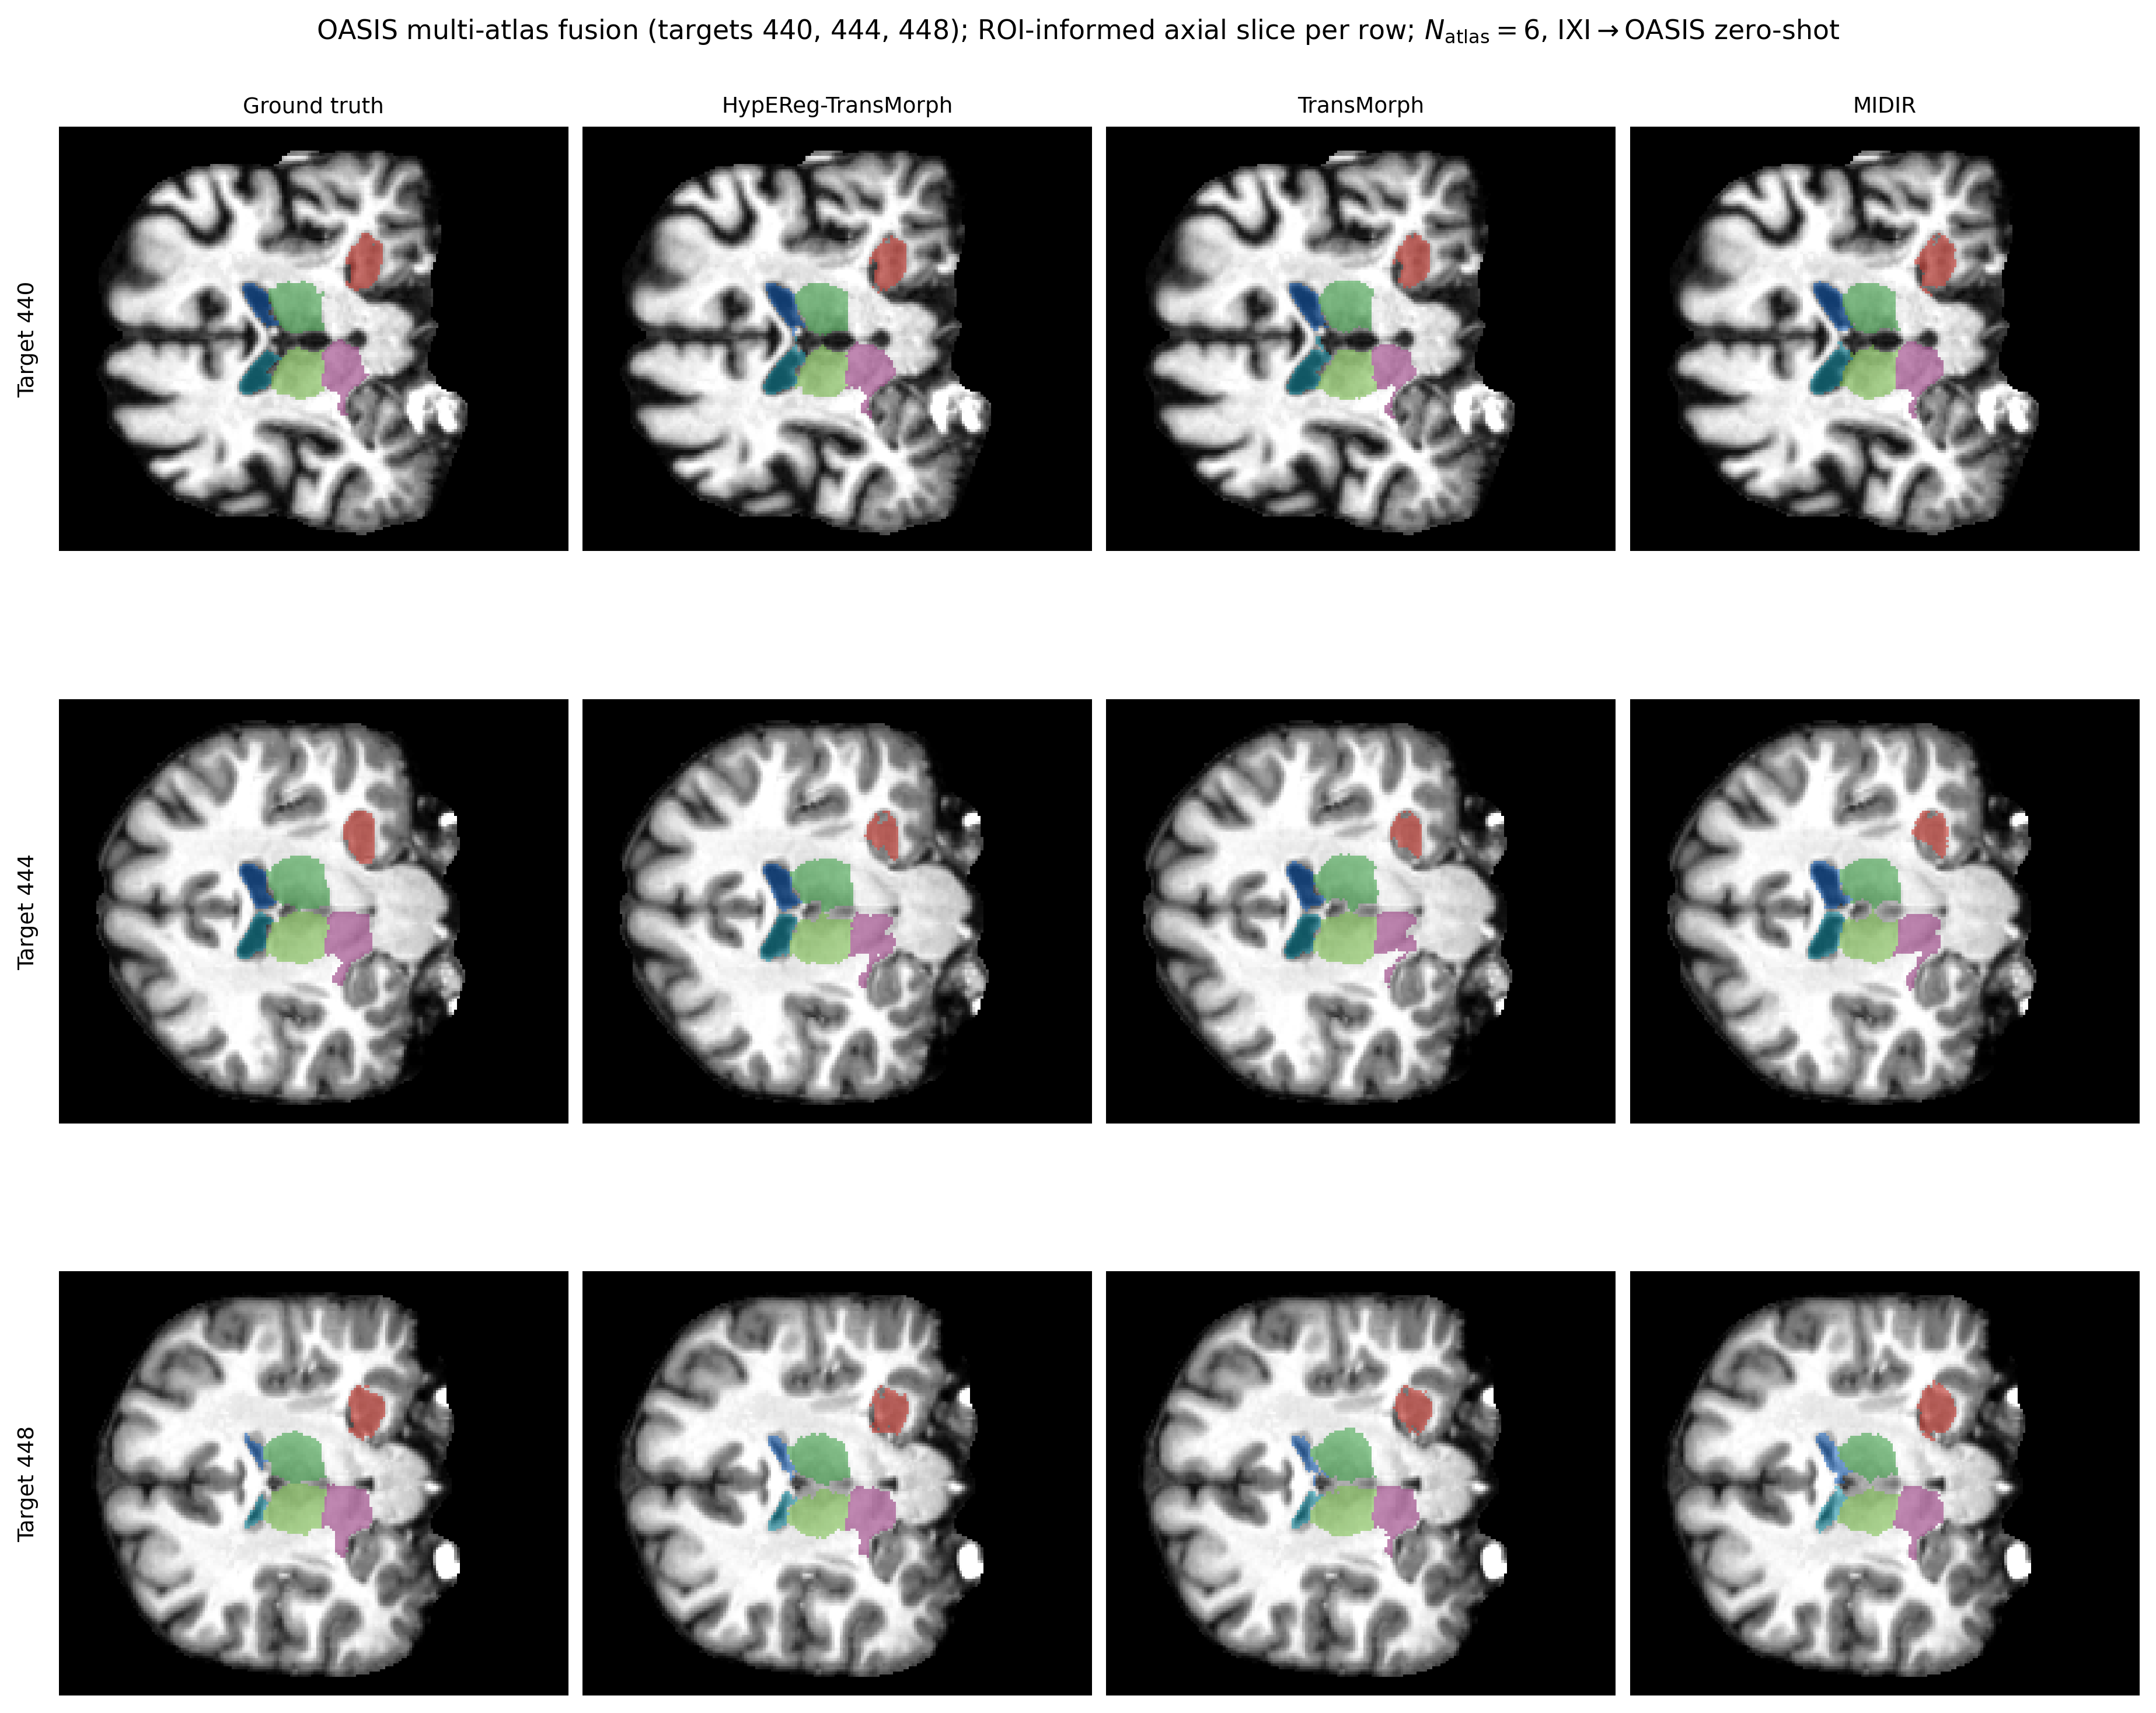
\includegraphics[width=0.98\textwidth]{figures/fig6_downstream_segmentation.png}
\caption{Qualitative downstream comparison on three OASIS test targets (rows) under strict IXI\(\to\)OASIS zero-shot inference. Columns: ground-truth structures (hippocampus, lateral ventricles, thalamus in distinct colours) and multi-atlas majority-voting fused segmentations (\(N_{\mathrm{atlas}}=6\)) from HypEReg-TransMorph, plain TransMorph, and MIDIR on the same T1 slice per row (slice chosen to maximize visibility of these ROIs). Fold-regularized HypEReg warps yield fused label maps closer to the reference than the unconstrained Transformer baseline, while MIDIR illustrates a structurally fold-free B-spline parameterization at lower absolute fused overlap (Table~\ref{tab:multiatlas}).\label{fig:downstream_segmentation}}
\end{figure}

%%%%%%%%%%%%%%%%%%%%%%%%%%%%%%%%%%%%%%%%%%
\section{Discussion}\label{sec:discussion}

\subsection{Primary Findings and Clinical Interpretation}
This work is framed as an improvement in deformation reliability rather than a narrow pursuit of overlap alone. Across IXI, HypEReg-TransMorph reduces non-positive Jacobian ratio and SDlogJ while preserving or improving overlap and surface metrics against strong Transformer baselines. This trade-off is clinically meaningful: deformation fields with high Dice but non-negligible folding are fundamentally problematic for Jacobian-based morphometry, longitudinal change analysis, and downstream label propagation.

The downstream multi-atlas experiment further supports this interpretation. In Section~\ref{sec:multiatlas}, HypEReg-TransMorph attains the highest fused Dice in zero-shot OASIS transfer (Table~\ref{tab:multiatlas}), and Figure~\ref{fig:downstream_segmentation} shows that this gain corresponds to visually cleaner, more anatomically coherent propagated labels in hippocampal, ventricular, and thalamic regions. In short, regularity improvements are not only mathematical; they transfer into application-level segmentation robustness.

\subsection{Comparison with MIDIR: Accuracy, Generalization, and Efficiency}
MIDIR is a particularly strong comparator because it guarantees fold-free transforms through B-spline parameterization and is computationally efficient. In our IXI evaluation, however, HypEReg-TransMorph remains superior in accuracy-related endpoints: grouped Dice is higher (0.7537 vs.\ 0.7423), ASSD is lower with significant paired differences, and HD95 is statistically comparable. This pattern indicates that architectural fold prevention alone does not guarantee best anatomical correspondence.

The gap widens under strict IXI\(\to\)OASIS transfer. HypEReg-TransMorph maintains a larger advantage in Dice and surface metrics, suggesting that loss-side Jacobian supervision combined with dense-flow Transformer expressivity adapts better to cohort shift than a fixed-grid spline parameterization. MIDIR still offers a real efficiency advantage (lower latency and much smaller parameter count), so the practical choice is deployment-dependent: MIDIR is attractive under hard compute constraints, whereas HypEReg-TransMorph is preferable when cross-domain fidelity and fusion quality are priority targets.

\subsection{Mechanistic Positioning and Portability}
HypEReg's main engineering advantage is that it acts on the training objective, not the inference graph. Fold suppression is learned through explicit determinant-level penalties, while runtime architecture, parameter count, and feed-forward speed remain unchanged relative to the underlying TransMorph backbone. This makes HypEReg portable to other dense-flow Transformer designs without re-architecting deployment pipelines.

Conceptually, this is complementary to methods that emphasize different structural constraints, including inverse-consistency objectives (ICON/GradICON) and hierarchical composition strategies (e.g., LapIRN) \cite{greer2021icon,tian2023gradicon,mok2020lapirn}. Those methods target cycle consistency or multi-scale deformation composition; HypEReg directly targets \(\det J_\phi\). Combining these ideas is therefore plausible rather than contradictory.

\subsection{Relation to Prior Hyperelastic Regularization}
Relative to prior hyperelastic-style regularizers, HypEReg is distinguished by operating directly at the Jacobian determinant level with a coupled design: a clamped-rational volume-distortion term plus an explicit anti-folding hinge. The selective Jacobian penalty in \citet{mok2020fast} is closest to the hinge component, but does not provide the same non-linear stabilization away from folding regimes. BMR-inspired volume-change/curvature regularization \cite{hering2021lung} and conformal-invariant energy approaches \cite{zou2023conformal} are important precedents, mostly demonstrated in CNN-dominant lung CT contexts. Our contribution is to show determinant-level non-linear regularization in a Transformer dense-flow brain MRI setting with paired inferential analysis at subject level.

\subsection{Limitations and Future Work}
Several limitations remain. First, the headline IXI comparison is based on single-run training per method; robustness is strengthened through subject-level paired non-parametric testing, but a full multi-seed training budget is still pending. Second, clinical impact is inferred through surrogate endpoints (Jacobian cleanliness, overlap/surface metrics, and downstream fusion), not direct reader-study outcomes or biomarker decision studies. Third, although strict zero-shot IXI\(\to\)OASIS and OASIS-retrained supplementary analyses provide evidence of cross-cohort behavior, broader pathology-rich external validation remains necessary.

Future work should prioritize (i) full multi-seed retraining with uncertainty decomposition, (ii) additional external cohorts and multimodal protocols, (iii) hybrid formulations that couple HypEReg with inverse-consistent or hierarchical objectives, and (iv) task-level clinical studies quantifying how fold suppression changes biomarker sensitivity, diagnostic confidence, and workflow time.

%%%%%%%%%%%%%%%%%%%%%%%%%%%%%%%%%%%%%%%%%%
\section{Conclusions}\label{sec:conclusion}

We have introduced HypEReg, a non-linear hyperelastic regularizer that couples a clamped-rational volume-distortion term with an explicit anti-folding hinge and acts directly on the Jacobian determinant of the predicted displacement field. Integrated into a TransMorph dense-flow backbone, the regularizer produces HypEReg-TransMorph, a learned brain MRI registration model that delivers near-diffeomorphic deformations at zero inference cost. On the IXI atlas-to-subject benchmark with 115 held-out test subjects, HypEReg-TransMorph reduces the non-positive Jacobian-determinant ratio by approximately three orders of magnitude relative to TransMorph and TransMorphBayes (1.502\% \(\to\) 0.0015\%), reduces SDlogJ from 0.5064 to 0.3280, improves grouped Dice over TransMorph (0.7537 vs.\ 0.7527) and significantly reduces ASSD (1.357\,mm vs.\ 1.407\,mm for TransMorph), while adding no inference latency or parameter overhead (Table~\ref{tab3}). A strict IXI\(\to\)OASIS zero-shot evaluation confirms that HypEReg-TransMorph attains the highest Dice and the lowest non-positive Jacobian ratio in the zero-shot group---roughly two orders of magnitude below plain TransMorph zero-shot (Section~\ref{sec:oasis_zs}; Table~\ref{tab:oasis_zeroshot}; Figure~\ref{fig:oasis_jacobian}). The regularity advantage extends to downstream clinical-style pipelines insofar as multi-atlas label fusion on OASIS (Section~\ref{sec:multiatlas}; Table~\ref{tab:multiatlas}) shows improved fused overlap when folding is suppressed, consistent with more consistent per-atlas label propagation.

These results address a long-standing usability gap of learning-based registration: Jacobian-based biomarkers, atlas-fusion segmentation, and longitudinal morphometry pipelines all assume one-to-one, fold-free warps, an assumption that unconstrained Transformer backbones routinely violate. By delivering near-diffeomorphic fields at feed-forward inference speed and without changes to the deployment architecture, HypEReg-TransMorph is a practical drop-in upgrade for Transformer-based deformable brain MRI registration. With the released open-source package and planned multi-seed retraining and additional external cohort experiments, non-linear Jacobian-aware regularization is positioned as a low-cost building block for improved deformation reliability.

%%%%%%%%%%%%%%%%%%%%%%%%%%%%%%%%%%%%%%%%%%
\vspace{6pt}

%%%%%%%%%%%%%%%%%%%%%%%%%%%%%%%%%%%%%%%%%%
\supplementary{The following supporting information can be downloaded with this article: Figure~S1, descriptive IXI multi-metric bar-chart overview; Figure~S2, qualitative registration comparisons across axial/coronal/sagittal views; Table~S1, IXI baseline checkpoint provenance; Table~S2, auxiliary IXI deformation/surface metrics (including NSD@1\,mm); Table~S3, IXI paired inferential summary (mean\(\pm\)std and aligned median tests); Table~S4, IXI paired Wilcoxon/BH-FDR results with effect sizes; Table~S5, grouped-VOI label mapping; Table~S6, OASIS-retrained paired Wilcoxon/BH-FDR results (distinct from main-text zero-shot); Table~S7, bootstrap 95\% confidence intervals on IXI subject-level means; Text~S1, OASIS retraining environment notes and implementation/profiling details.}

%%%%%%%%%%%%%%%%%%%%%%%%%%%%%%%%%%%%%%%%%%
\funding{This research received no external funding.}

\institutionalreview{Not applicable. This study performed secondary analysis of publicly available anonymized IXI data and did not recruit new human participants.}

\informedconsent{Not applicable to this secondary-analysis study using publicly available anonymized data.}

\dataavailability{Source code, configuration files, per-case metric tables, and figure/statistics scripts are openly available at \url{https://github.com/Zzxmh/HypEReg-TransMorph} and archived at Zenodo: \url{https://doi.org/10.5281/zenodo.19888526} \cite{xu2026hypereg_zenodo}. Trained model weights will be deposited alongside the published artifact. The IXI dataset used in this study is publicly available at \url{https://brain-development.org/ixi-dataset/} (CC BY-SA 3.0). The preprocessed split follows the public TransMorph-style IXI preprocessing release.}

\conflictsofinterest{The authors declare no conflicts of interest.}

%%%%%%%%%%%%%%%%%%%%%%%%%%%%%%%%%%%%%%%%%%
\abbreviations{Abbreviations}{
The following abbreviations are used in this manuscript:
\\
\noindent
\begin{tabular}{@{}ll}
HypEReg & Hyperelastic-Energy Regularization\\
MRI & Magnetic Resonance Imaging\\
HD95 & 95th percentile Hausdorff Distance\\
ASSD & Average Symmetric Surface Distance\\
NCC & Normalized Cross-Correlation\\
LNCC & Local Normalized Cross-Correlation\\
SDlogJ & Standard Deviation of Log Jacobian Determinant\\
IXI & Information eXtraction from Images dataset\\
BMR & Burger--Modersitzki--Ruthotto (hyperelastic energy framework)\\
FDR & False Discovery Rate
\end{tabular}
}

%%%%%%%%%%%%%%%%%%%%%%%%%%%%%%%%%%%%%%%%%%
\begin{adjustwidth}{-\extralength}{0cm}

\reftitle{References}

%=====================================
% References, variant A: external bibliography
%=====================================
\bibliography{refs}

\PublishersNote{}
\end{adjustwidth}
\end{document}





